Nous avons vu au chapitre \ref{chap:cosmo1} que la fonction de masse prédisait l'abondance de halos de matière sombre par unité de masse et de redshift.
Étant donné le lien étroit entre le processus de formation des structures et la cosmologie sous-jacente, on peut prédire que la fonction de masse dépend des propriétés de l'Univers et de son évolution depuis l'inflation.
Elle fait donc le lien entre la distribution de matière dans l'Univers et les paramètres cosmologiques à travers l'abondance de surdensités par unités de masse et de redshift.

C'est dans ce contexte que les amas de galaxies apparaissent comme une sonde cosmologique.
Ils constituent en effet les plus grandes structures gravitationnellement liées de l'Univers, et apparaissent comme l'aboutissement du processus de formation hiérarchique des structures.
Le nombre d'amas de galaxies observables dans le ciel est donc directement lié à la fonction de masse.
Par conséquent, un catalogue d'amas de galaxies de masse et redshift connus permet de   contraindre la fonction de masse, et donc les paramètres cosmologiques.

Ce chapitre décrit les éléments nécessaires à la réalisation de telles analyses.
Nous nous intéresserons tout d'abord à la définition des amas de galaxies et à leurs caractéristiques.
Nous discuterons ensuite des différentes observables des amas dans différentes longueurs d'onde, puis des contraintes cosmologiques par comptage d'amas de galaxies.
Nous terminerons par un tour d'horizon des résultats récents en cosmologie avec des amas de galaxies, et des perspectives de ce domaine.

% ===================================================================================== %
\section{Composition et masse des amas de galaxies}

% ------------------------------------------------------------------------------------- %
\subsection{Définition d'un amas de galaxies}

Les amas de galaxies représentent la dernière étape du processus de formation hiérarchique des structures développé dans la section \ref{sec:struct_form}, et constituent les plus grandes structures gravitationnellement liées de l'Univers.
Ils se forment par effondrement gravitationnel de la matière et par accrétion du milieu environnant autour des pics de densité de la toile cosmique, c'est-à-dire aux intersections de ses filaments.
Ils offrent donc un traceur de la distribution de matière dans l'Univers.
C'est la raison pour laquelle leur distribution en masse et en redshift constitue une sonde permettant d'étudier les processus de formation des structures, et donc la cosmologie sous-jacente.
Ce point sera abordé plus en détail en section \ref{sec:cluster_nbcount}.

La formation des amas de galaxies a lieu dans l'Univers contemporain, à des redshifts $z \lesssim 3$.
Les structures de plus haut redshift sont essentiellement représentées par des galaxies seules, ou par des groupes d'un petit nombre de galaxies, désignés comme proto-amas (voir par exemple \cite{zhou_goods-alma_2020}).

La composition des amas de galaxies est représentative de celle de la matière dans l'Univers (voir \eg\ \cite{pratt_galaxy_2019}).
Elle est dominée par la matière sombre, comptant pour $\sim$ 85 \% de leur masse.
La matière baryonique des amas est principalement contenue dans un gaz chaud ionisé nommé milieu intra-amas (ou ICM pour \textit{intracluster medium}), représentant $\sim$ 12 \% du contenu en masse des amas.
Ce gaz est principalement composé de noyaux légers et d'électrons libres, à des températures de l'ordre de $10^7 - 10^8 \;{\rm K}$.
Enfin, le reste de la matière baryonique des amas est contenu dans leurs galaxies, qui ne représentent qu'une faible fraction de la masse totale des amas ($\sim$ 3\%).

% ------------------------------------------------------------------------------------- %
\subsection{Masse et rayon des amas de galaxies} \label{sec:int_quant}

Les amas de galaxies sont des objets complexes et diffus par nature, auxquels il est difficile d'attribuer une taille physique.
Leur étude passe donc par la définition d'un rayon caractéristique à l'intérieur duquel leurs propriétés physiques seront étudiées.
Pour cela, le rayon de viriel peut être utilisé, décrivant un halo à l'équilibre.
En pratique, celui-ci est difficile à estimer, du fait des différents processus physiques perturbant leur équilibre, et de sa taille souvent plus grande que les champs couverts par les observations.
Par conséquent, il est plus utile de définir un rayon $R_\Delta$ par la valeur moyenne du contraste de densité $\Delta$ qu'il contient:
\begin{equation}
    \label{eq:cluster_contrast_R}
    \Delta \equiv \frac{\left<\rho(<R_\Delta)\right>}{\rho_{\rm crit}(z)},
\end{equation}
ce qui correspond à considérer l'amas comme une boule homogène de masse volumique $\Delta$ fois supérieure à la densité critique de l'Univers. \\
La valeur de contraste considérée est arbitraire; les valeurs usuelles sont $\Delta \in [200, 500, 2500]$, en fonction de la couverture angulaire des observations utilisées et des régions d'intérêt.
Des études portant sur les propriétés des amas dans $R_{2500}$ se focaliseront sur le cœur des amas, alors que des études à $R_{200}$ permettront des contraintes sur leur périphérie.
Au cours de cette thèse, nous utiliserons principalement $R_{500}$, valeur conventionnellement utilisée pour des études sur les régions intermédiaires des amas de galaxies et du milieu intra-amas.
Comme nous le verrons en section \mypageref{sec:current_surveys}, les amas de galaxies détectés par les instruments actuels ont des masses $M_{500}$ typiquement de l'ordre de $10^{14} - 10^{15} \;M_\odot$.

Parmi les propriétés fondamentales des amas de galaxies, leur masse joue un rôle crucial dans l'estimation de contraintes sur les paramètres cosmologiques.
La connaissance des masses individuelles d'un grand nombre d'amas de galaxies est en effet nécessaire aux études de comptage, qui constituent l'une des sondes cosmologiques majeures basées sur les amas de galaxies, et qui sera détaillée en section \ref{sec:cluster_nbcount}.

Plusieurs méthodes existent pour estimer la masse d'amas individuels; nous renvoyons le lecteur vers la revue récente de \myciteauthor{pratt_galaxy_2019} pour une liste détaillée des différentes possibilités ouvertes par les observations récentes d'amas de galaxies à différentes longueurs d'onde.
La mesure principale utilisée dans cette thèse repose sur la connaissance des propriétés thermodynamiques du milieu intra-amas, et sur l'hypothèse de l'équilibre hydrostatique.
Dans le cadre de cette hypothèse, les forces gravitationnelles subies par un élément de fluide sont compensées par les forces de pression:
\begin{equation}
    \frac{1}{\rho} \vec{\nabla} P = \vec{g} = \frac{-G M^{\rm HSE}}{r^2} \vec{u}_r,
\end{equation}
où $\vec{u}_r$ est un vecteur unitaire radial en coordonnées sphériques. \\
Alors, dans l'hypothèse de symétrie sphérique de l'amas, le profil de masse, soit la valeur de masse contenue dans une sphère de rayon $r$, s'écrit
\begin{equation}
    \label{eq:mhse}
    M^{\rm HSE}(<r) = \frac{-r^2}{G \mu m_{\rm p} n_\e(r)} \frac{\d P_\e}{\d r},
\end{equation}
où $\mu$ est le poids moléculaire moyen du milieu intra-amas, $\mu \equiv m/m_{\rm p}$; et $n_\e(r)$ et $P_\e(r)$ sont respectivement la densité et la pression des électrons du milieu intra-amas. \\
L'hypothèse de l'équilibre hydrostatique offre donc un estimateur du profil de masse des amas de galaxies.
La masse $M_\Delta$ contenue dans un rayon $R_\Delta$ peut alors être estimée grâce à la connaissance du profil de masse d'un amas de galaxies.
En effet, le rayon $R_\Delta$ peut être calculé en considérant une boule homogène de rayon $R_\Delta$ et de masse volumique $\rho_c(z)$, soit en résolvant:
\begin{equation}
    \label{eq:r_delta_from_m}
    \frac{M(<R_\Delta)}{\rho_c(z) \times \frac{4}{3} \pi R_\Delta^3} = \Delta.
\end{equation}
La valeur du profil de masse à ce rayon donne donc la masse $M_\Delta = M(<R_\Delta)$.
On note au passage la corrélation entre $R_\Delta$ et $M_\Delta$ par construction. Ce point revêt une importance capitale pour les mesures de relations d'échelle masse-observable, et sera discuté dans les chapitres \ref{chap:panco} et \ref{chap:scaling}.

La masse hydrostatique se présente donc comme un estimateur de la masse d'un amas reposant sur la mesure du profil de densité et de pression des électrons de l'ICM.
Comme nous le verrons par la suite, il est possible de mesurer ces propriétés grâce à l'émission des amas de galaxies en X et à l'observation de l'effet Sunyaev-Zeldovich.

% ------------------------------------------------------------------------------------- %
\subsection{Le biais hydrostatique}\label{sec:hse_bias}

La validité de l'hypothèse de l'équilibre hydrostatique dans les amas est le sujet de nombreuses études (\eg\ \cite{salvati_mass_2019}).
En effet, comme nous le verrons par la suite, les analyses cosmologiques par comptage d'amas sont limitées par la connaissance des masses des amas.
Une grande variété des processus physiques ayant lieu au sein de ces derniers (fusion de sous-structures, injection d'énergie par des noyaux actifs de galaxies) créent dans le milieu intra-amas des forces de pression non-thermiques.
Celles-ci ne sont en général pas contraintes par les observations, comme nous le verrons par la suite.
Les masses estimées par observation des propriétés thermodynamiques du milieu intra-amas peuvent donc souffrir d'un biais.
Celui-ci est nommé biais hydrostatique $b$, et permet de quantifier l'état de perturbation des amas:
\begin{equation}
    \label{eq:hse_bias}
    M^{\rm HSE} = (1-b)M^{\rm total}.
\end{equation}
On remarque alors que ce biais se propage au profil de masse hydrostatique discuté dans la section précédente, et donc au calcul du rayon caractéristique $R_\Delta$ décrit dans l'équation (\ref{eq:r_delta_from_m}).
La masse caractéristique $M_\Delta$ obtenue grâce au profil de masse hydrostatique est donc affectée de ce biais non-seulement de par la différence entre les profils de masse, mais également par la différence des rayons caractéristiques inférés.

La mesure du biais hydrostatique peut être réalisée par plusieurs moyens.
On peut étudier le biais à partir de simulations hydrodynamiques, dans lesquelles la masse réelle des amas est connue et la masse hydrostatique peut être calculée à partir de l'équation (\ref{eq:mhse}) (\eg\ \cite{barnes_characterizing_2021,gianfagna_exploring_2021}).
Cependant, cette approche suppose que les simulations sont parfaitement réalistes, et les résultats dépendent fortement de la modélisation des différents processus physiques inclus dans les simulations utilisées \cite{gianfagna_exploring_2021}.
Le biais hydrostatique peut également être étudié à partir d'observations.
En effet, il existe plusieurs estimateurs de masse des amas qui ne reposent pas sur l'hypothèse de l'équilibre hydrostatique.
Par exemple, les mesures de masse par effet de lentillage gravitationnel du CMB (\eg\ \cite{madhavacheril_atacama_2020, louis_calibrating_2017, zubeldia_cosmological_2019}) ou de galaxies d'arrière-plan\footnotemark (\eg\ \cite{sereno_comparing_2015}).
Les différents estimateurs de masse peuvent être comparés sur des échantillons d'amas afin de mesurer l'écart moyen entre les mesures de masse hydrostatique et celles ne reposant pas sur cette hypothèse.
\footnotetext{Plus de détails seront donnés en section \mypageref{sec:opt}.}

Une compilation de mesures de $(1-b)$ est présentée en figure \ref{fig:hse_bias}, montrant les différentes valeurs de biais obtenues par comparaison d'estimateurs de masse à partir d'observations et de simulations.
La région orange montre la valeur du biais hydrostatique obtenue par l'analyse cosmologique jointe des observations par \textit{Planck} de l'effet Sunyaev-Zeldovich et du CMB réalisée par \myciteauthor{salvati_constraints_2018}.
Une tension apparait: ce résultat est incompatible avec les mesures de biais réalisées par la comparaison de différents estimateurs de masse d'amas observés, à partir d'observations (points noirs) et de simulations (région violette).
S'il est à noter que cette différence a récemment été réduite par la réanalyse des observations du CMB par \textit{Planck}\footnotemark, la détermination de la valeur du biais hydrostatique reste l'un des enjeux majeurs de la cosmologie avec des amas de galaxies.
En effet, elle peut avoir un impact prononcé sur les mesures de paramètres cosmologiques, et une mauvaise estimation de $b$ entraîne un biais sur la mesure du paramètre $S_8$ (introduit en \ref{sec:cosmo_hmf}, et qui sera discuté en \ref{sec:current_surveys}).
\footnotetext{En particulier, la valeur de la profondeur optique jusqu'à la réionisation, $\tau$, a évolué entre les analyses de la collaboration \textit{Planck} en 2015 et 2018. Plus de détails peuvent être trouvés dans \cite{planck_collaboration_planck_2020}.}

\begin{SCfigure}[][t]
    \centering
    \includegraphics[width=.4\linewidth]{Figures/Chap_amas/b_salvati.eps}
    \hspace{15pt}
    \caption{
        Estimation du biais hydrostatique par comparaison de mesures de masse hydrostatique et par lentillage faible (voir section \ref{sec:opt}) pour différentes études (noir).
        La valeur nécessaire pour concilier les réultats du CMB et des amas de galaxies, mesurée par \cite{salvati_constraints_2018}, est indiquée en orange.
        La région violette représente les valeurs de $(1-b)$ permises par plusieurs analyses d'amas simulés \cite{planck_collaboration_planck_2013}.
        Figure extraite de \cite{salvati_constraints_2018}.
    }
    \label{fig:hse_bias}
\end{SCfigure}

% ===================================================================================== %
\section{Observations des amas de galaxies} \label{sec:cluster_obs}

La richesse des processus physiques ayant lieu au sein des amas de galaxies font de ceux-ci des objets multilongueur d'onde par nature, pouvant être détectés dans tous des domaines du spectre électromagnétique.
Dans cette section, nous présentons les longueurs d'onde principales utilisées pour la caractérisation des amas de galaxies, ainsi que les propriétés physiques des amas qu'elles permettent respectivement de sonder.
Une attention particulière sera portée à l'effet Sunyaev-Zeldovich, qui constitue l'observable principale étudiée au cours de cette thèse, en \ref{sec:sz}.

À titre d'illustration, les cartes d'un amas de galaxies dans les trois domaines de longueur d'onde discutés ici sont présentées en figure \ref{fig:macsj1149}.
On y voit que les amas apparaissent comme des objets diffus dans les observations dans les domaines millimétrique et X.
Comme nous le verrons par la suite, la raison en est que de telles observations cartographient le gaz du milieu intra-amas; c'est pourquoi la structure des amas à ces longueurs d'onde sont souvent similaires.
Les observations en visible des amas révèlent quant à elles la distribution des galaxies membres de l'amas.

\afterpage{
\begin{figure*}[t]
    \centering
    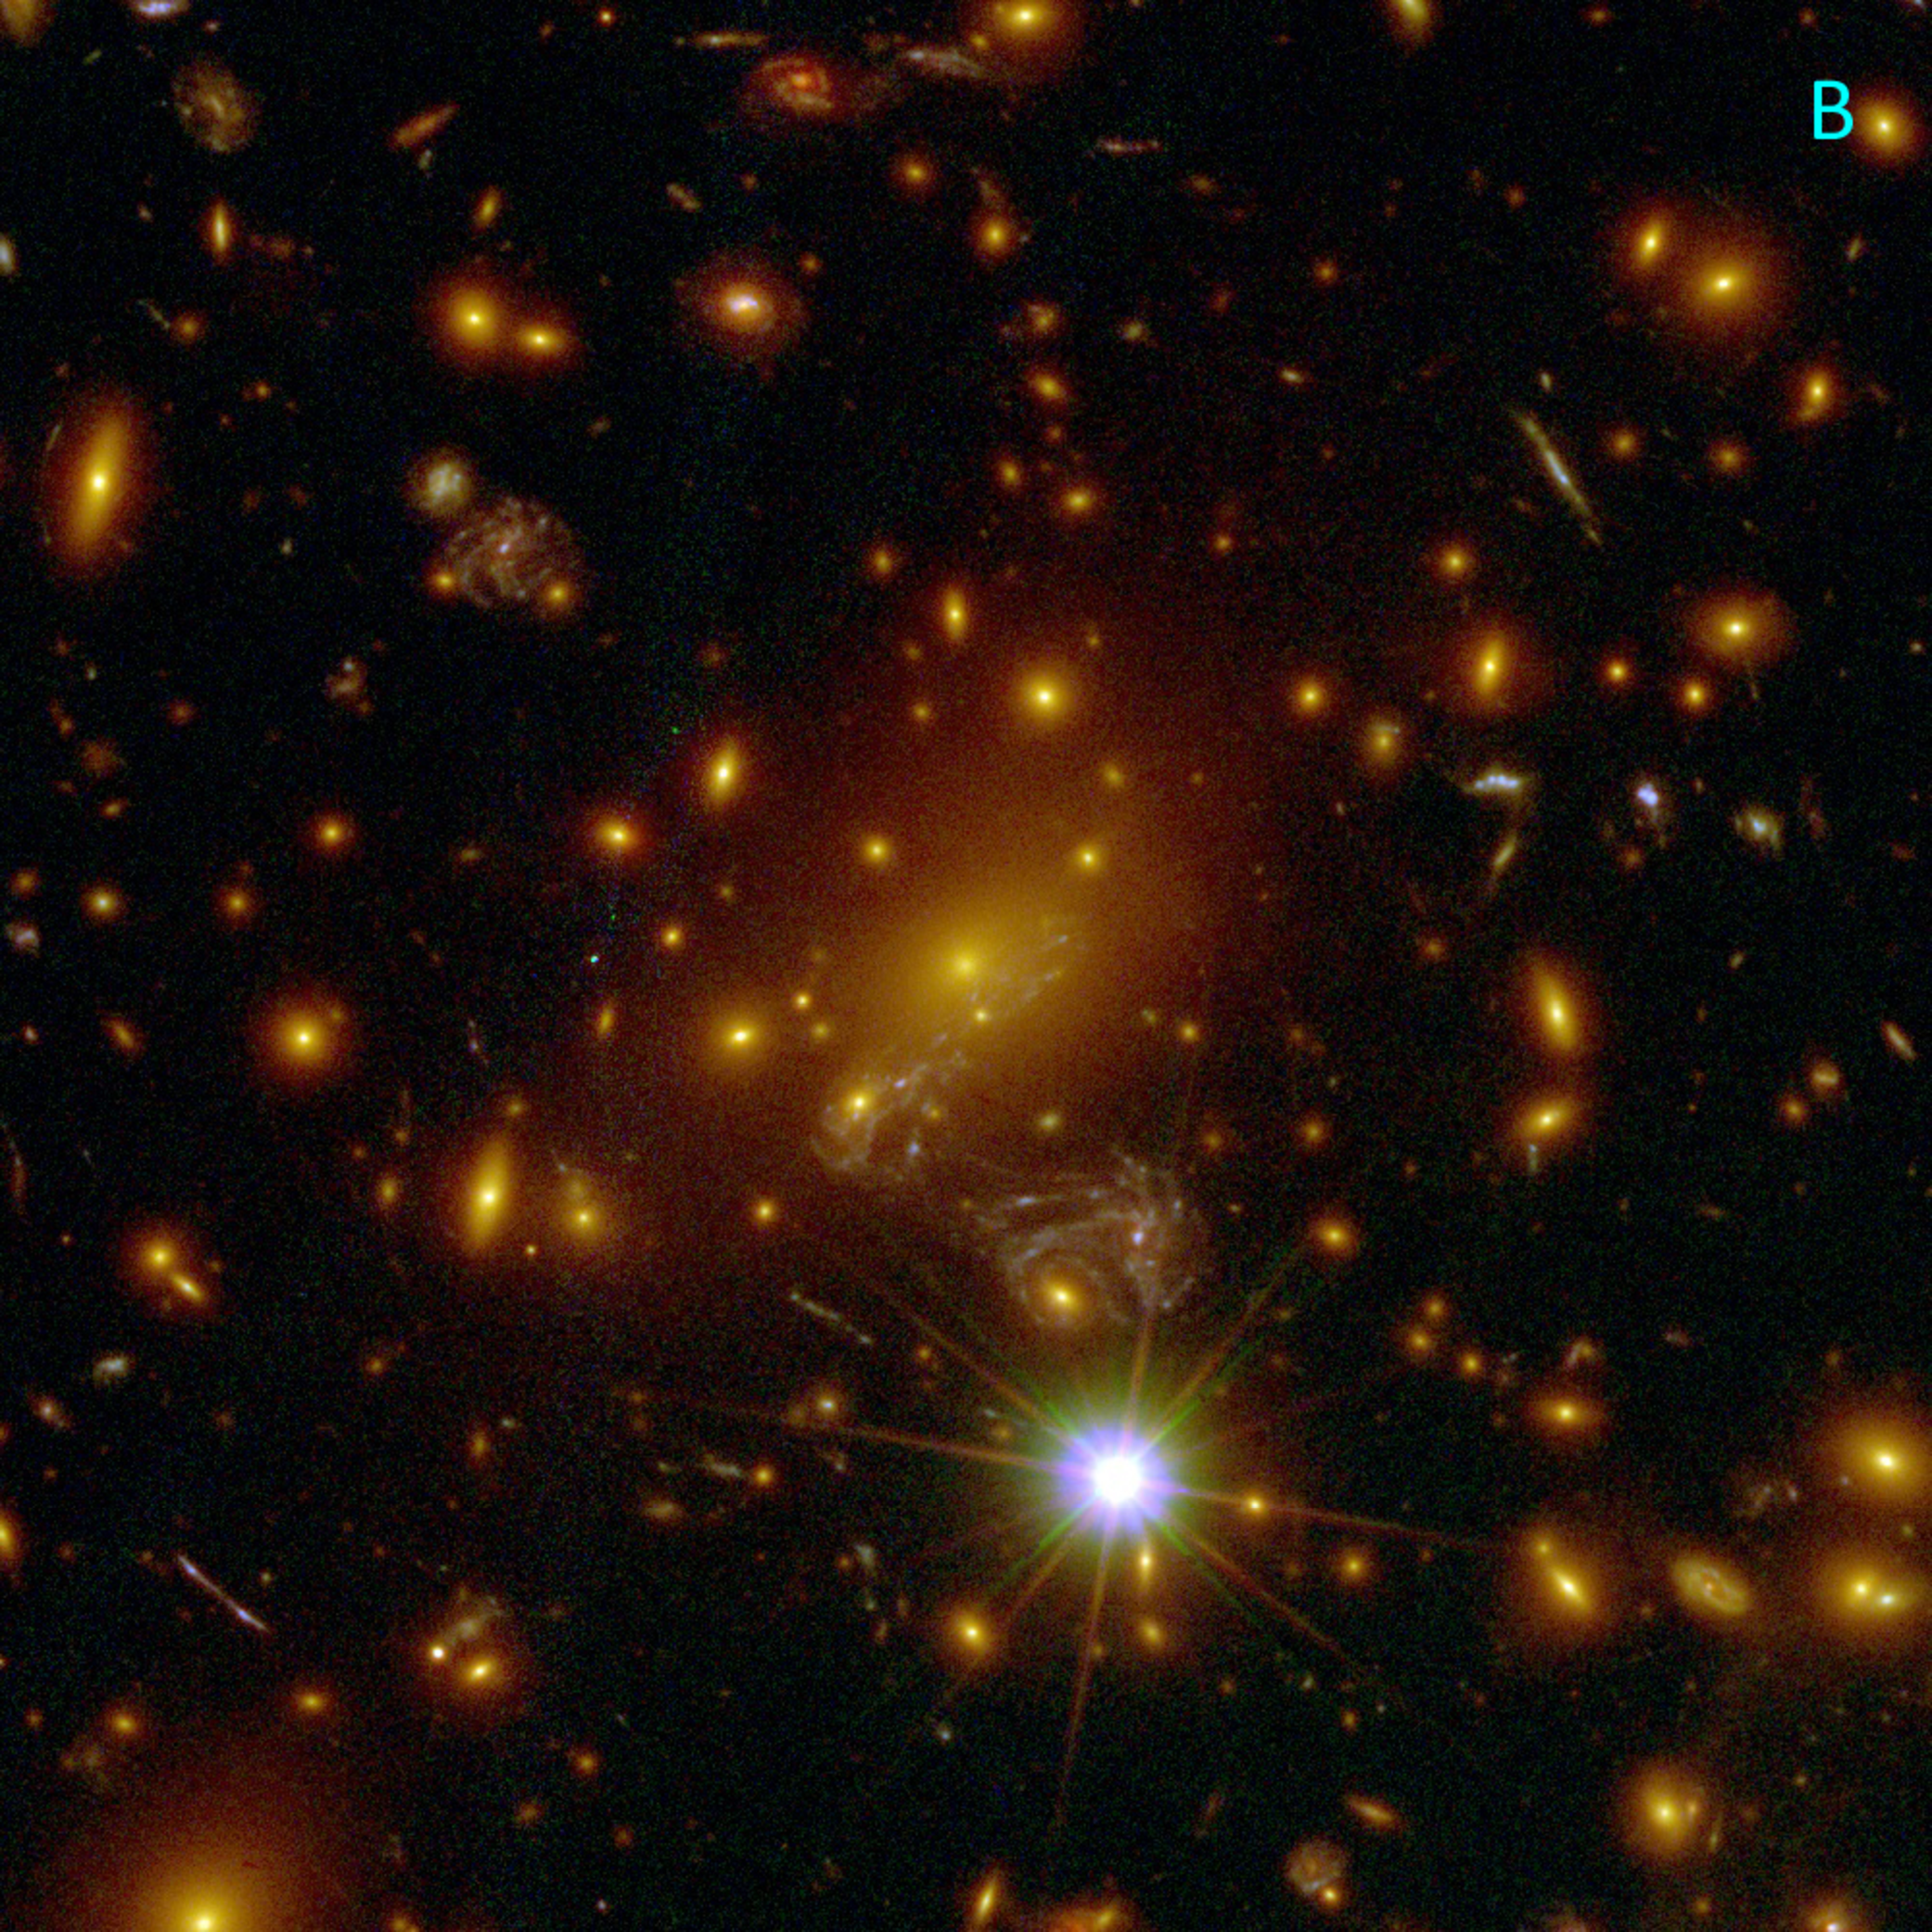
\includegraphics[width=.3\linewidth]{Figures/Chap_amas/macsj1149_opt.pdf}\hspace{10pt}
    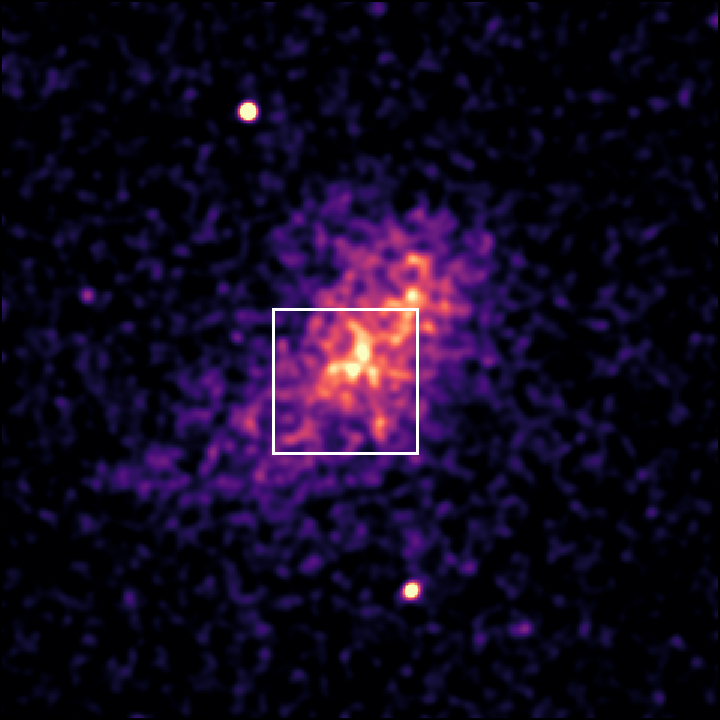
\includegraphics[width=.3\linewidth]{Figures/Chap_amas/macsj1149_X_frame.pdf}\hspace{10pt}
    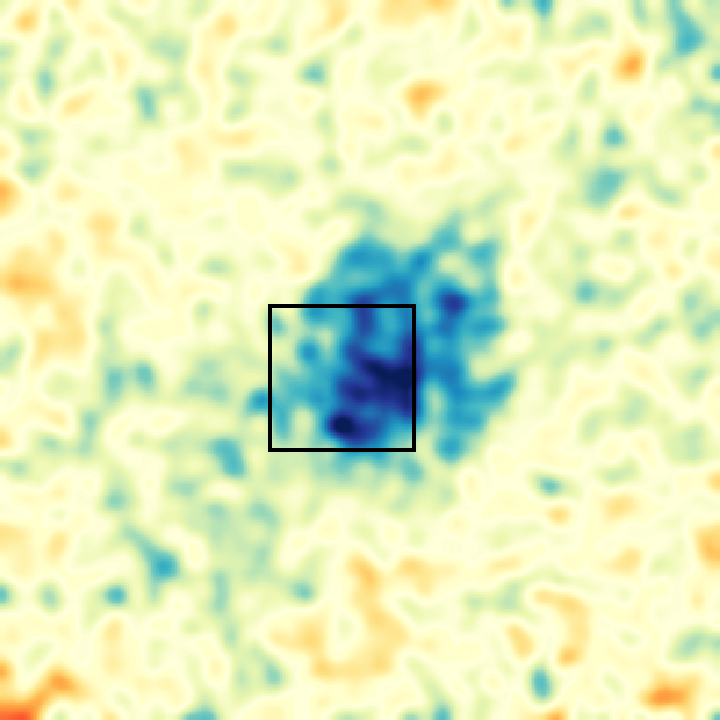
\includegraphics[width=.3\linewidth]{Figures/Chap_amas/macsj1149_SZ_frame.pdf}
    \caption{
        Cartographie de l'amas de galaxies MACSJ1149.5+2223 par le \textit{Hubble Space Telescope} en optique et infrarouge (\textit{gauche}, extraite de \cite{postman_cluster_2012}), en X avec \textit{Chandra} (\textit{centre}), et en millimétrique par l'effet Sunyaev-Zeldovich avec NIKA2 (\textit{droite}).
        La taille de la région cartographiée est de 1 arcmin pour la carte optique, et de 5 arcmin pour les cartes X et SZ.
        La région cartographiée en optique est représentée par un carré sur les cartes X et SZ.
    }
    \label{fig:macsj1149}
\end{figure*}
}

% ------------------------------------------------------------------------------------- %
\subsection{Observations en visible et infrarouge}\label{sec:opt}

De la première détection d'un amas de galaxies à la fin du 18$^\e$ siècle à l'avènement des premiers satellites X dans la deuxième moitié du 20$^\e$ siècle, les amas de galaxies étaient uniquement observés dans des longueurs d'ondes visibles \cite{biviano_messier_2000}.
L'émission visible et infrarouge des amas provient de leur composante stellaire, contenue dans les galaxies membres des amas.
Elle peut être étudiée par observations photométriques ou spectroscopiques, donnant chacune accès à des informations différentes sur les amas de galaxies observés.

Les mesures photométriques, basées sur l'acquisition d'images du ciel dans différentes bandes de longueurs d'onde, permettent l'étude des images des galaxies du champ.
La position de ces galaxies dans un diagramme couleur-magnitude permet de séparer les galaxies membres de l'amas de celles d'avant- ou arrière-plan; c'est sur ce principe que sont basés certains algorithmes de détection des amas en optique, par exemple redMaPPer \cite{rykoff_redmapper_2014}.
D'autres algorithmes existent, notamment basés sur la géométrie de la distribution de galaxies (voir par exemple \cite{adam_euclid_2019}).
La distribution des galaxies membres peut être utilisée comme un traceur du potentiel gravitationnel, offrant des contraintes sur la distribution de masse et sur l'état dynamique des amas.
En particulier, la richesse d'un amas, définie comme le nombre de galaxies membres observables, fait partie des observables étroitement liées à la masse des amas (cf. section \ref{sec:scaling}).
Elle est par conséquent fréquemment utilisée dans les relevés optiques pour estimer la masse d'amas pour lesquels des mesures individuelles de masse ne sont pas possibles\footnote{Voir par exemple \cite{costanzi_cosmological_2021,phriksee_weak_2020} pour des résultats récents.}.

L'étude des galaxies d'arrière-plan offre la possibilité de mesurer la masse d'un amas grâce au lentillage gravitationnel.
En effet, les photons en provenance de ces sources distantes sont déviés par le fort potentiel gravitationnel des amas, résultant en des distorsions de leurs images.
Ces distorsions peuvent être séparées en deux grands régimes.
Dans le cas de faibles distorsions, souvent caractérisées par une simple déformation des galaxies d'arrière-plan, on parle de lentillage gravitationnel faible (ou \textit{weak lensing}).
Celui-ci n'est souvent détectable que par étude statistique des déformations des galaxies d'arrière-plan, ne permettant pas toujours une mesure des masses individuelles des amas de galaxies (voir \cite{umetsu_clustergalaxy_2020} pour une revue sur le lentillage faible autour des amas).
Le régime de lentillage fort (ou \textit{strong lensing}) est quant à lui caractérisé par l'apparition de plusieurs images d'une même galaxie d'arrière-plan, ou bien d'une déformation extrême comme l'apparition darcs, ou plus rarement d'anneaux d'Einstein.
Il permet alors une étude plus détaillée de la distribution du potentiel gravitationnel au sein d'amas individuels.
Le lentillage gravitationnel n'est pas nécessairement présent et détectable autour d'un amas de galaxies.
En particulier, il nécessite la présence de sources d'arrière-plan, qui sont plus rares pour les amas distants, limitant le potentiel des mesures de masses par lentillage à haut redshift.
De plus, les mesures de déformations des galaxies d'arrière-plan sont fortement affectées par des effets systématiques, de par le fait qu'elles requièrent des hypothèses sur la forme réelle de ces galaxies, et qu'elles dépendent fortement des conditions d'observations et des caractéristiques des instruments utilisés (\eg\ \cite{becker_accuracy_2011,mandelbaum_instrumental_2015,grandis_calibration_2021,sommer_weak_2021}).
Ainsi, si les estimations de masses des amas ne sont pas biaisées\footnotemark, elles sont en général plus dispersées que les estimations basées sur les mesures des propriétés thermodynamiques du milieu intra-amas (\cite{pratt_galaxy_2019,umetsu_clustergalaxy_2020,grandis_calibration_2021}).
\footnotetext{Au sens où elles mesurent la masse gravitationnelle de l'amas sans reposer sur l'hypothèse de l'équilibre hydrostatique; elles sont toutefois affectées d'autres biais -- voir \eg\ \cite{pratt_galaxy_2019,grandis_calibration_2021,sommer_weak_2021}.}

Enfin, les amas de galaxies peuvent être observés aux longueurs d'onde visibles et infrarouges par spectroscopie.
Ce sont alors les spectres des galaxies qui sont mesurés, c'est-à-dire l'évolution de leur flux avec la fréquence.
De tels relevés sont capables de mesurer les redshifts des galaxies des amas, à l'aide de l'identification des longueurs d'onde observées de raies spectrales connues.
Les observations spectroscopiques d'amas de galaxies offrent aussi un moyen d'estimer la dispersion des vitesses des galaxies membres par mesure de l'effet Doppler.
Cette dispersion étant liée à la distribution de masse dans les amas, elle peut également être utilisée comme observable reliée à la masse pour des analyses cosmologiques (\eg\ \cite{munari_relation_2013, ferragamo_biases_2020}).

Plusieurs grands relevés dans les domaines visible et infrarouge sont sur le point de commencer; par exemple, le Legacy Survey of Space and Time réalisé par le Vera Rubin Observatory \cite{lsst_science_collaboration_lsst_2009} et le relevé \textit{Euclid} \cite{amendola_cosmology_2013}.
Il est prévu que ces deux relevés détectent un nombre d'amas supérieur de plusieurs ordres de grandeurs au nombre d'amas actuellement connus, avec des mesures de masses par lentillage d'une grande qualité grâce aux performances des instruments \cite{lsst_dark_energy_science_collaboration_large_2012,sartoris_next_2016}.

% ------------------------------------------------------------------------------------- %
\subsection{Observations en X}\label{sec:x}

L'un des domaines de longueur d'onde couramment utilisés pour l'étude des amas de galaxies est le domaine des rayons X.
Les amas de galaxies sont émetteurs en X principalement au travers du rayonnement de freinage (\textit{bremsstrahlung}) des électrons dans le gaz chaud du milieu intra-amas (voir \cite{bohringer_x-ray_2013} pour une revue).
La brillance de surface observée en direction d'un amas $S_X$ est liée aux propriétés thermodynamiques du milieu intra-amas:
\begin{equation}
    \label{eq:x_brightness}
    S_X = \frac{1}{4\pi (1+z)^4} \int \Lambda(T_\e, Z) \, n_\e^2 \, \d l,
\end{equation}
où $n_\e$ est la densité des électrons du milieu intra-amas, et $\Lambda(T_\e, Z)$ est la fonction de refroidissement dépendant de la température des électrons du milieu $T_\e$ et de sa métallicité $Z$, quantifiant l'abondance d'éléments plus lourds que l'hélium dans le milieu intra-amas. \\
La fonction de refroidissement peut être déterminée par étude spectroscopique du signal X, qui sera détaillée au prochain paragraphe.
L'intégration a lieu le long de la ligne de visée $l$.
Comme le montre l'équation (\ref{eq:x_brightness}), l'amplitude du signal X mesuré en direction d'un amas renseigne sur la densité d'électrons présente le long de la ligne de visée considérée.
Les observations d'amas en X permettent donc la mesure de la distribution des électrons dans le milieu intra-amas, nécessaire au calcul de la masse détaillé plus tôt (équation \ref{eq:mhse}).

En plus du continuum d'émission X due au \textit{bremsstrahlung} thermique des électrons, l'émission X dans le milieu intra-amas comporte des raies spectrales caractéristiques des transitions entre niveaux d'énergie des éléments présents dans le gaz.
Lorsqu'une observation d'un amas a permis d'accumuler suffisamment de photons X, ils est alors possible d'étudier leur distribution en énergie, qui représente le spectre du milieu intra-amas.
La connaissance de ce spectre permet de quantifier l'abondance des éléments émettant les raies spectrales étudiées, et donc la métallicité $Z$ de l'amas.
De plus, le spectre étant intimement lié à la température des électrons du gaz, les études de spectroscopie X permettent également de la mesurer\footnote{Voir \cite{bohringer_x-ray_2010} pour une revue de la spectroscopie X}.
Ainsi, des observations profondes d'amas de galaxies en X permettent de mesurer à la fois la densité et la température électronique du milieu intra-amas.
Ce milieu étant très dilué, avec des densités rarement supérieures à $10^{-2}$ électrons par centimètre cube, il peut être modélisé comme un gaz parfait.
Les mesures de densité et de pression peuvent alors être combinées pour obtenir une estimation de la pression électronique:
\begin{equation}
    \label{eq:pvnrt}
    P_\e = n_\e k_\textsc{b} T_\e,
\end{equation}
qui peut à son tour être combinée à la densité d'électrons pour calculer la masse des amas par l'équation (\ref{eq:mhse}).

Étant donnée l'opacité de l'atmosphère aux rayons X, les observations d'amas à ces longueurs d'onde ne peuvent être réalisées que depuis des satellites.
La plupart des études d'amas de galaxies en X font actuellement appel à des mesures avec les satellites \textit{XMM-Newton} \cite{jansen_xmm-newton_2001} et \textit{Chandra} \cite{weisskopf_overview_2002}.
Dans le futur, les mesures spectroscopiques fournies par la mission \textit{Athena} \cite{nandra_hot_2013} permettront la caractérisation des propriétés du milieu intra-amas avec une grande précision.
L'émission X des amas peut également être utilisée pour créer des catalogues d'amas, comme le relevé actuellement réalisé par l'instrument eROSITA \cite{merloni_erosita_2012} qui permettra la détection de plusieurs centaines de milliers d'amas.

Ainsi, l'étude du rayonnement X des amas de galaxies permet de mesurer les propriétés thermodynamiques de leur milieu intra-amas, jusqu'à leur masse, de manière autonome et sans avoir à recourir à des observations dans d'autres longueurs d'onde.
Il est toutefois à noter que l'analyse spectroscopique des photons X en provenance d'amas recquiert des observations très profondes, et est donc particulièrement coûteuse en temps.
C'est l'une des raisons qui motive la combinaison d'observations X peu profondes, ne permettant de mesurer que la distribution de densité du milieu intra-amas, avec des observations effectuées à d'autres longueurs d'onde, sensibles à d'autres propriétés physiques.
C'est par exemple le cas de l'effet Sunyaev-Zeldovich, détaillé dans la section suivante.


% ------------------------------------------------------------------------------------- %
\subsection{Observations en millimétrique: l'effet Sunyaev-Zeldovich}\label{sec:sz}

L'effet Sunyaev-Zeldovich (SZ, \cite{zeldovich_interaction_1969, sunyaev_interaction_1970,sunyaev_observations_1972,sunyaev_velocity_1980}) est une distorsion du fond diffus cosmologique due à l'interaction de ses photons avec les électrons des amas de galaxies.
L'interaction ayant lieu est une diffusion Compton inverse: les photons du CMB, peu énergétiques ($\sim 10^{-6} \;{\rm keV}$ lors de la formation des amas, à $z \lesssim 3$), diffusent sur les électrons libres du milieu intra-amas.
Ces derniers possédant une grande énergie cinétique, les photons acquièrent de l'énergie, modifiant la forme du spectre observé du CMB dans la direction des amas.

L'effet SZ peut être séparé en plusieurs composantes, parfois considérées comme des effets SZ différents, selon le processus physique à l'origine de l'énergie cinétique des électrons transmise aux photons du CMB.
Dans chacun des cas, le gain en énergie est lié aux propriétés physiques du milieu intra-amas, et l'observation des effets SZ permet de mesurer ces propriétés et donc de caractériser la physique des amas de galaxies.
Nous listons ici les trois effets SZ les plus fréquemment utilisés: l'effet SZ thermique (tSZ), cinétique (kSZ) et relativiste (rSZ).
Des revues détaillées des différents effets SZ et de leur utilisation en astrophysique et cosmologie peuvent être trouvées, par exemple, dans \cite{birkinshaw_sunyaevzeldovich_1999,carlstrom_cosmology_2002,mroczkowski_astrophysics_2019}.

\subsubsection{L'effet Sunyaev-Zeldovich thermique} % --------------------------------- %
Le milieu intra-amas est composé d'un gaz chaud ionisé, dont la température est généralement de l'ordre de $10^7 - 10^8 \;{\rm K}$.
Dans l'hypothèse d'un gaz parfait, ces températures correspondent à une énergie d'agitation thermique $3 k_\textsc{b} T / 2$ de l'ordre de $1-10 \;{\rm keV}$, bien supérieure à l'énergie des photons du CMB.
La diffusion de Compton inverse permet alors aux électrons de céder une partie de cette énergie aux photons du CMB.

La dépendance spectrale de la distorsion peut être calculée à partir de l'équation de Kompaneets \cite{kompaneets_establishment_1957, freire_oliveira_derivation_2021}: pour un bain d'électrons non-relativistes ($k_\textsc{b} T_\e \ll m_\e c^2$) traversé par des photons de fréquence réduite $x_\e \equiv h\nu/k_\textsc{b} T_\e$, on a
\begin{equation}
    \label{eq:kompaneets}
    \pdv{n}{y} = \frac{1}{x_\e^2}\pdv{}{x_\e} \left[ x_\e^4\left( \pdv{n}{x_\e} + n^2 + n \right) \right],
\end{equation}
où $n$ est l'indice d'occupation des photons, défini pour une intensité spécifique $I_\nu$ à une fréquence $\nu$ comme
\begin{equation}
    n \equiv \frac{I_\nu c^2}{2 h \nu^3},
\end{equation}
et $y$ est le paramètre de Compton, défini comme
\begin{equation}
    y \equiv \int \frac{k_\textsc{b} T_\e}{m_\e c^2} \, \d\tau_\e
\end{equation}
où $\tau_\e \equiv n_\e \sigma_\textsc{t} l$ est la profondeur optique\footnotemark\ parcourue par les photons le long de la ligne de visée $l$; $n_\e$ est la densité d'électrons, et $\sigma_\textsc{t}$ la section efficace de diffusion Thompson. \\
\footnotetext{Dans l'hypothèse d'un milieu optiquement mince.}
Cette équation peut alors aussi s'écrire
\begin{equation}
    \label{eq:sz_y}
    y = \int \frac{k_\textsc{b} T_\e}{m_\e c^2} n_\e \sigma_\textsc{t} \, \d l
      = \frac{\sigma_\textsc{t}}{m_\e c^2} \int k_\textsc{b} T_\e \, n_\e \, \d l.
\end{equation}
Dans le cas de l'effet SZ, l'énergie des photons incidents est très faible par rapport à celle des électrons, soit $x_\e \ll 1$ et donc $\partial n / \partial x_\e \gg n, n^2$.
L'équation (\ref{eq:kompaneets}) se simplifie alors, et en y injectant l'expression d'un spectre de corps noir pour les photons du CMB, on trouve l'expression de la variation d'intensité spécifique due à l'effet tSZ:
\begin{equation}
    \label{eq:sz_dI}
    \frac{\Delta I_\nu^{\rm tSZ}}{I_0} = y \times \frac{x^4 e^x}{(e^x - 1)^2} \big[ x \, {\rm coth}(x/2) - 4 \big] \big[ 1 + \delta_r(x, T) \big],
\end{equation}
où $x \equiv h\nu / k_\textsc{b}T_\textsc{cmb}$, et $\delta_r(x, T)$ traduit les corrections relativistes à l'effet tSZ, qui seront discutées par la suite, et $I_0 \equiv 2(k_\textsc{b} T_\textsc{cmb})^3 / (hc)^2$ est l'intensité spécifique du CMB.

\begin{figure*}[t]
    \centering
    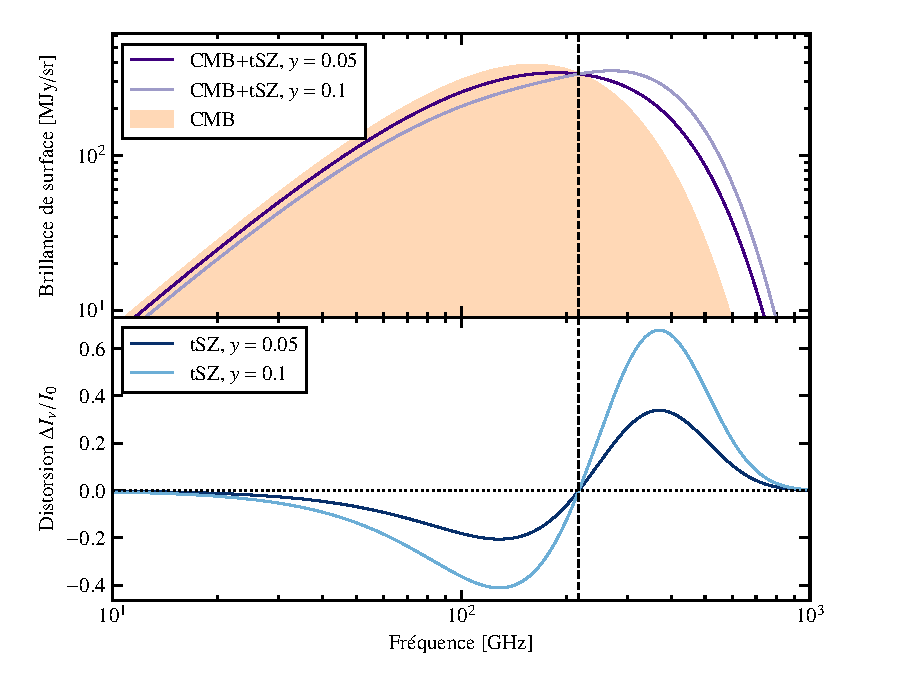
\includegraphics[width=.8\linewidth]{Figures/Chap_amas/CMB_SZ_spectrum.pdf}
    \caption{
        \textbf{Haut:} Spectre des photons du CMB (orange) et de photons ayant interagi avec un amas pour deux valeurs de paramètres de Compton $y$ (violet).
        Au premier ordre, l'effet tSZ représente un décalage du spectre vers les grandes fréquences.
        \textbf{Bas:} Distorsion spectrale due à l'effet tSZ pour les mêmes valeurs de paramètre de Compton.
        La signature observationnelle de l'effet tSZ apparaît comme un décrément dans la brillance de surface du CMB aux fréquences inférieures à 217 GHz (ligne noire verticale), et un incrément au-delà.
        Les valeurs de paramètre de Compton utilisées sont grandement exagérées pour des raisons visuelles.
        Les corrections relativistes à l'effet tSZ sont négligées.
    }
    \label{fig:tsz_spec}
\end{figure*}

La distorsion spectrale due à l'effet tSZ est représentée sur la figure \ref{fig:tsz_spec}.
On peut voir sur le panneau haut que le spectre de photons ayant interagi par effet tSZ est décalé vers les grandes fréquences, correspondant à un gain d'énergie par diffusion Compton inverse.
Le panneau bas montre la distorsion spectrale relative provoquée par l'effet tSZ (équation \ref{eq:sz_dI}).
Celle-ci se manifeste par un déficit de photons de basse énergie, et une augmentation du nombre de photons à haute énergie, par rapport au spectre du CMB avant interaction.
Ainsi, en observant le fond diffus cosmologique en direction d'amas de galaxies, on détectera un décrément dans sa brillance de surface aux fréquences inférieures à 217 GHz, et un incrément aux fréquences supérieures.
Cette signature spectrale est très caractéristique de l'effet tSZ, et permet de le différencier des autres sources astrophysiques, comme nous le verrons en \ref{sec:current_surveys}.

D'après l'équation (\ref{eq:sz_dI}), l'amplitude de la distorsion due à l'effet tSZ est donnée par le paramètre de Compton $y$.
Ce lien est également illustré en figure \ref{fig:tsz_spec}, montrant un incrément et un décrément plus importants pour des valeurs de $y$ plus élevées.
En supposant que le gaz chaud du milieu intra-amas est bien décrit par un gaz parfait (hypothèse discutée en \ref{sec:x}), l'expression du paramètre de Compton (équation \ref{eq:sz_y}) prend la forme:
\begin{equation}
    \label{}
    y(\theta) = \frac{\sigma_\textsc{t}}{m_\e c^2} \int P_\e \, \d l(\theta),
\end{equation}
où $\theta$ représente les coordonnées observées dans le ciel, et $P_\e$ est la pression due aux électrons, donnée par l'équation (\ref{eq:pvnrt}). \\
La cartographie de l'effet SZ en direction d'amas de galaxies permet donc de mesurer la distribution de pression électronique dans le milieu intra-amas.

Comme le montre l'équation (\ref{eq:sz_y}), l'amplitude de la distorsion spectrale due à l'effet tSZ ne dépend pas du redshift des amas.
Cette indépendance permet à l'effet tSZ d'être l'un des moyens privilégiés pour la détection d'amas de galaxies distants.
En effet, alors même que la brillance de surface X décroît comme $(1+z)^{-4}$ (équation \ref{eq:x_brightness}), et que les amas distants sont composés de galaxies moins brillantes, un amas de galaxies de haut redshift ne sera pas moins brillant en millimétrique qu'un amas proche de même masse.
Les relevés d'amas de galaxies par effet SZ sont donc capables de détecter des amas plus distants et donc plus anciens que leurs équivalents optiques et X.
De plus, les observations de l'effet tSZ permettent la mesure du paramètre de Compton intégré $Y$,
\begin{equation}
    \label{eq:sz_yinteg}
    Y_\Delta = 4\pi\frac{\sigma_\textsc{t}}{m_\e c^2}\int_0^{R_\Delta} P_\e(r) \, r^2 \, \d r,
\end{equation}
qui représente une mesure du contenu en énergie thermique dans le milieu intra-amas.
Ainsi, l'effet tSZ permet la détection d'amas de galaxies distants, ainsi qu'une mesure de l'énergie contenue dans leur milieu intra-amas.

\subsubsection{L'effet Sunyaev-Zeldovich cinétique} % --------------------------------- %
En plus de l'énergie provenant de leur agitation thermique, les électrons libres du milieu intra-amas peuvent posséder une énergie cinétique du fait de mouvements d'ensemble du gaz.
Une partie de cette énergie peut alors se transmettre aux photons du CMB traversant le milieu intra-amas, provoquant l'effet SZ cinétique, ou kSZ \cite{sunyaev_velocity_1980}.
Contrairement à l'effet tSZ, le mouvement des électrons ne peut par construction pas être supposé isotrope.
La distorsion spectrale du CMB s'écrit alors
\begin{equation}
    \label{eq:ksz_dI}
    \frac{\Delta I_\nu^{\rm kSZ}}{I_0} = y_{\rm kSZ} \frac{x^4 e^x}{(e^x - 1)^2}\left[ 1 + \delta_r'(x, T, v_z) \right],
\end{equation}
où $\delta_r'$ représente les corrections relativistes à l'effet kSZ, discutées par la suite, et $v_z$ est la vitesse de déplacement du gaz le long de la ligne de visée, dont dépend l'amplitude de la distorsion dans une direction $\theta$:
\begin{equation}
    \label{eq:ksz_y}
    y_{\rm kSZ}(\theta) \equiv \frac{v_z(\theta)}{c} \int \d\tau_\e
    = \frac{\sigma_\textsc{t} v_z(\theta)}{c} \int n_\e(l) \,\d l(\theta).
\end{equation}

La comparaison des équations (\ref{eq:sz_dI}) et (\ref{eq:ksz_dI}) permet de mettre en évidence la différence entre les signatures spectrales des deux effets.
Celle-ci est illustrée en figure \ref{fig:ksz_spec}, montrant que l'effet kSZ peut se manifester comme un incrément ou un décrément en brillance de surface du CMB, selon la direction du déplacement de l'amas.
En effet, d'après les équations (\ref{eq:ksz_dI}) et (\ref{eq:ksz_y}), un mouvement de gaz en direction de l'observateur ($v_z > 0$) créera un incrément en brillance de surface, et à l'inverse, le gaz s'éloignant de l'observateur ($v_z < 0$) créera un décrément.
Ainsi par exemple, dans le cas d'un amas en rotation selon un axe non parallèle à la ligne de visée, l'effet kSZ se manifestera, à une même fréquence, comme un incrément dans les régions où le gaz s'approche de l'observateur, et comme un décrément dans les régions s'en éloignant.
On remarque enfin que le maximum de la distorsion due à l'effet kSZ se situe à la fréquence à laquelle celle de l'effet tSZ est nulle, c'est-à-dire $217 \;{\rm GHz}$.
Une mesure du ciel à cette fréquence permet donc \prior\ de mesurer l'effet kSZ sans contamination par le tSZ.
Cependant, pour les amas de grande extension spatiale -- proches et massifs -- l'effet kSZ est confondu avec les anisotropies primaires du CMB, du fait de la similarité entre les spectres de puissance de ces deux types d'anisotropie.

\begin{figure*}[t]
    \centering
    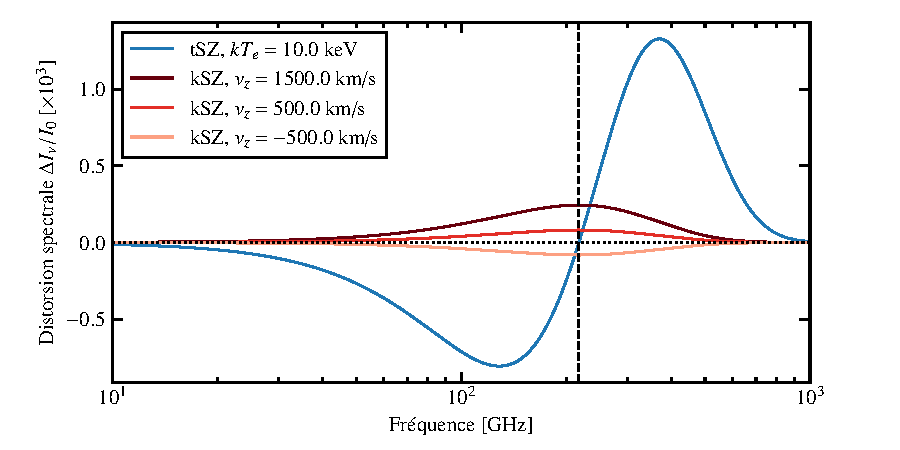
\includegraphics[width=.8\linewidth]{Figures/Chap_amas/tSZ_kSZ_spectrum.pdf}
    \caption{
        Signatures spectrales de l'effet tSZ (bleu) et kSZ (rouge) pour un amas de profondeur optique $\tau_\e = 10^{-2}$.
        L'amplitude de l'effet tSZ est calculée en supposant un milieu intra-amas isotherme avec $k_\textsc{b} T_\e = 10\;{\rm keV}$.
        Les amplitudes pour l'effet kSZ sont calculées pour différentes valeurs de vitesse le long de la ligne de visée.
        Dans les deux cas, les corrections relativistes sont négligées.
    }
    \label{fig:ksz_spec}
\end{figure*}

Comme le montre l'équation (\ref{eq:ksz_y}), la mesure de l'effet kSZ permet de mesurer le produit de la densité d'électrons et de la vitesse de déplacement du gaz.
En combinaison avec des mesures de champs de vitesses dans les amas réalisées en optique (cf. \ref{sec:opt}), l'effet kSZ offre donc l'opportunité de mesurer la densité du milieu intra-amas.
D'après l'équation (\ref{eq:mhse}), la combinaison des effets tSZ et kSZ peut donc fournir une mesure de la masse des amas dans l'hypothèse de l'équilibre hydrostatique.
Cependant, l'amplitude de l'effet kSZ est bien plus faible que celle de l'effet tSZ.
En effet, le rapport entre les deux est de l'ordre de $(k_\textsc{b} T_\e / m_\e c^2) / (v_z / c) \sim 10$ pour des vitesses de l'ordre de la centaine de km/s et des températures de l'ordre de la dizaine de keV (propriétés caractéristiques d'une grande majorité des amas de galaxies).
Cette différence d'amplitude entre les effets tSZ et kSZ pour des propriétés d'amas réalistes est visible sur la figure \ref{fig:krsz_spec}.

La mesure d'un signal kSZ significatif requiert donc une grande sensibilité, de même que des mesures à plusieurs longueurs d'onde pour pouvoir séparer sa contribution au signal total de celle de l'effet tSZ.
Des détections de l'effet kSZ existent, basées sur l'empilement de signaux en provenance de plusieurs amas (\eg\ \cite{hand_evidence_2012}) ou sur les mesures profondes d'amas dans lesquels des grandes vitesses de mouvements sont attendues (comme l'amas MACS~J0717.5+3745, \cite{mroczkowski_multi-wavelength_2012, adam_mapping_2017-1}).
Dans le cadre des observations traitées au cours de cette thèse, il est souvent négligeable: au vu du faible rapport signal sur bruit des observations, le niveau de signal kSZ sera inférieur au bruit.

\begin{figure*}[t]
    \centering
    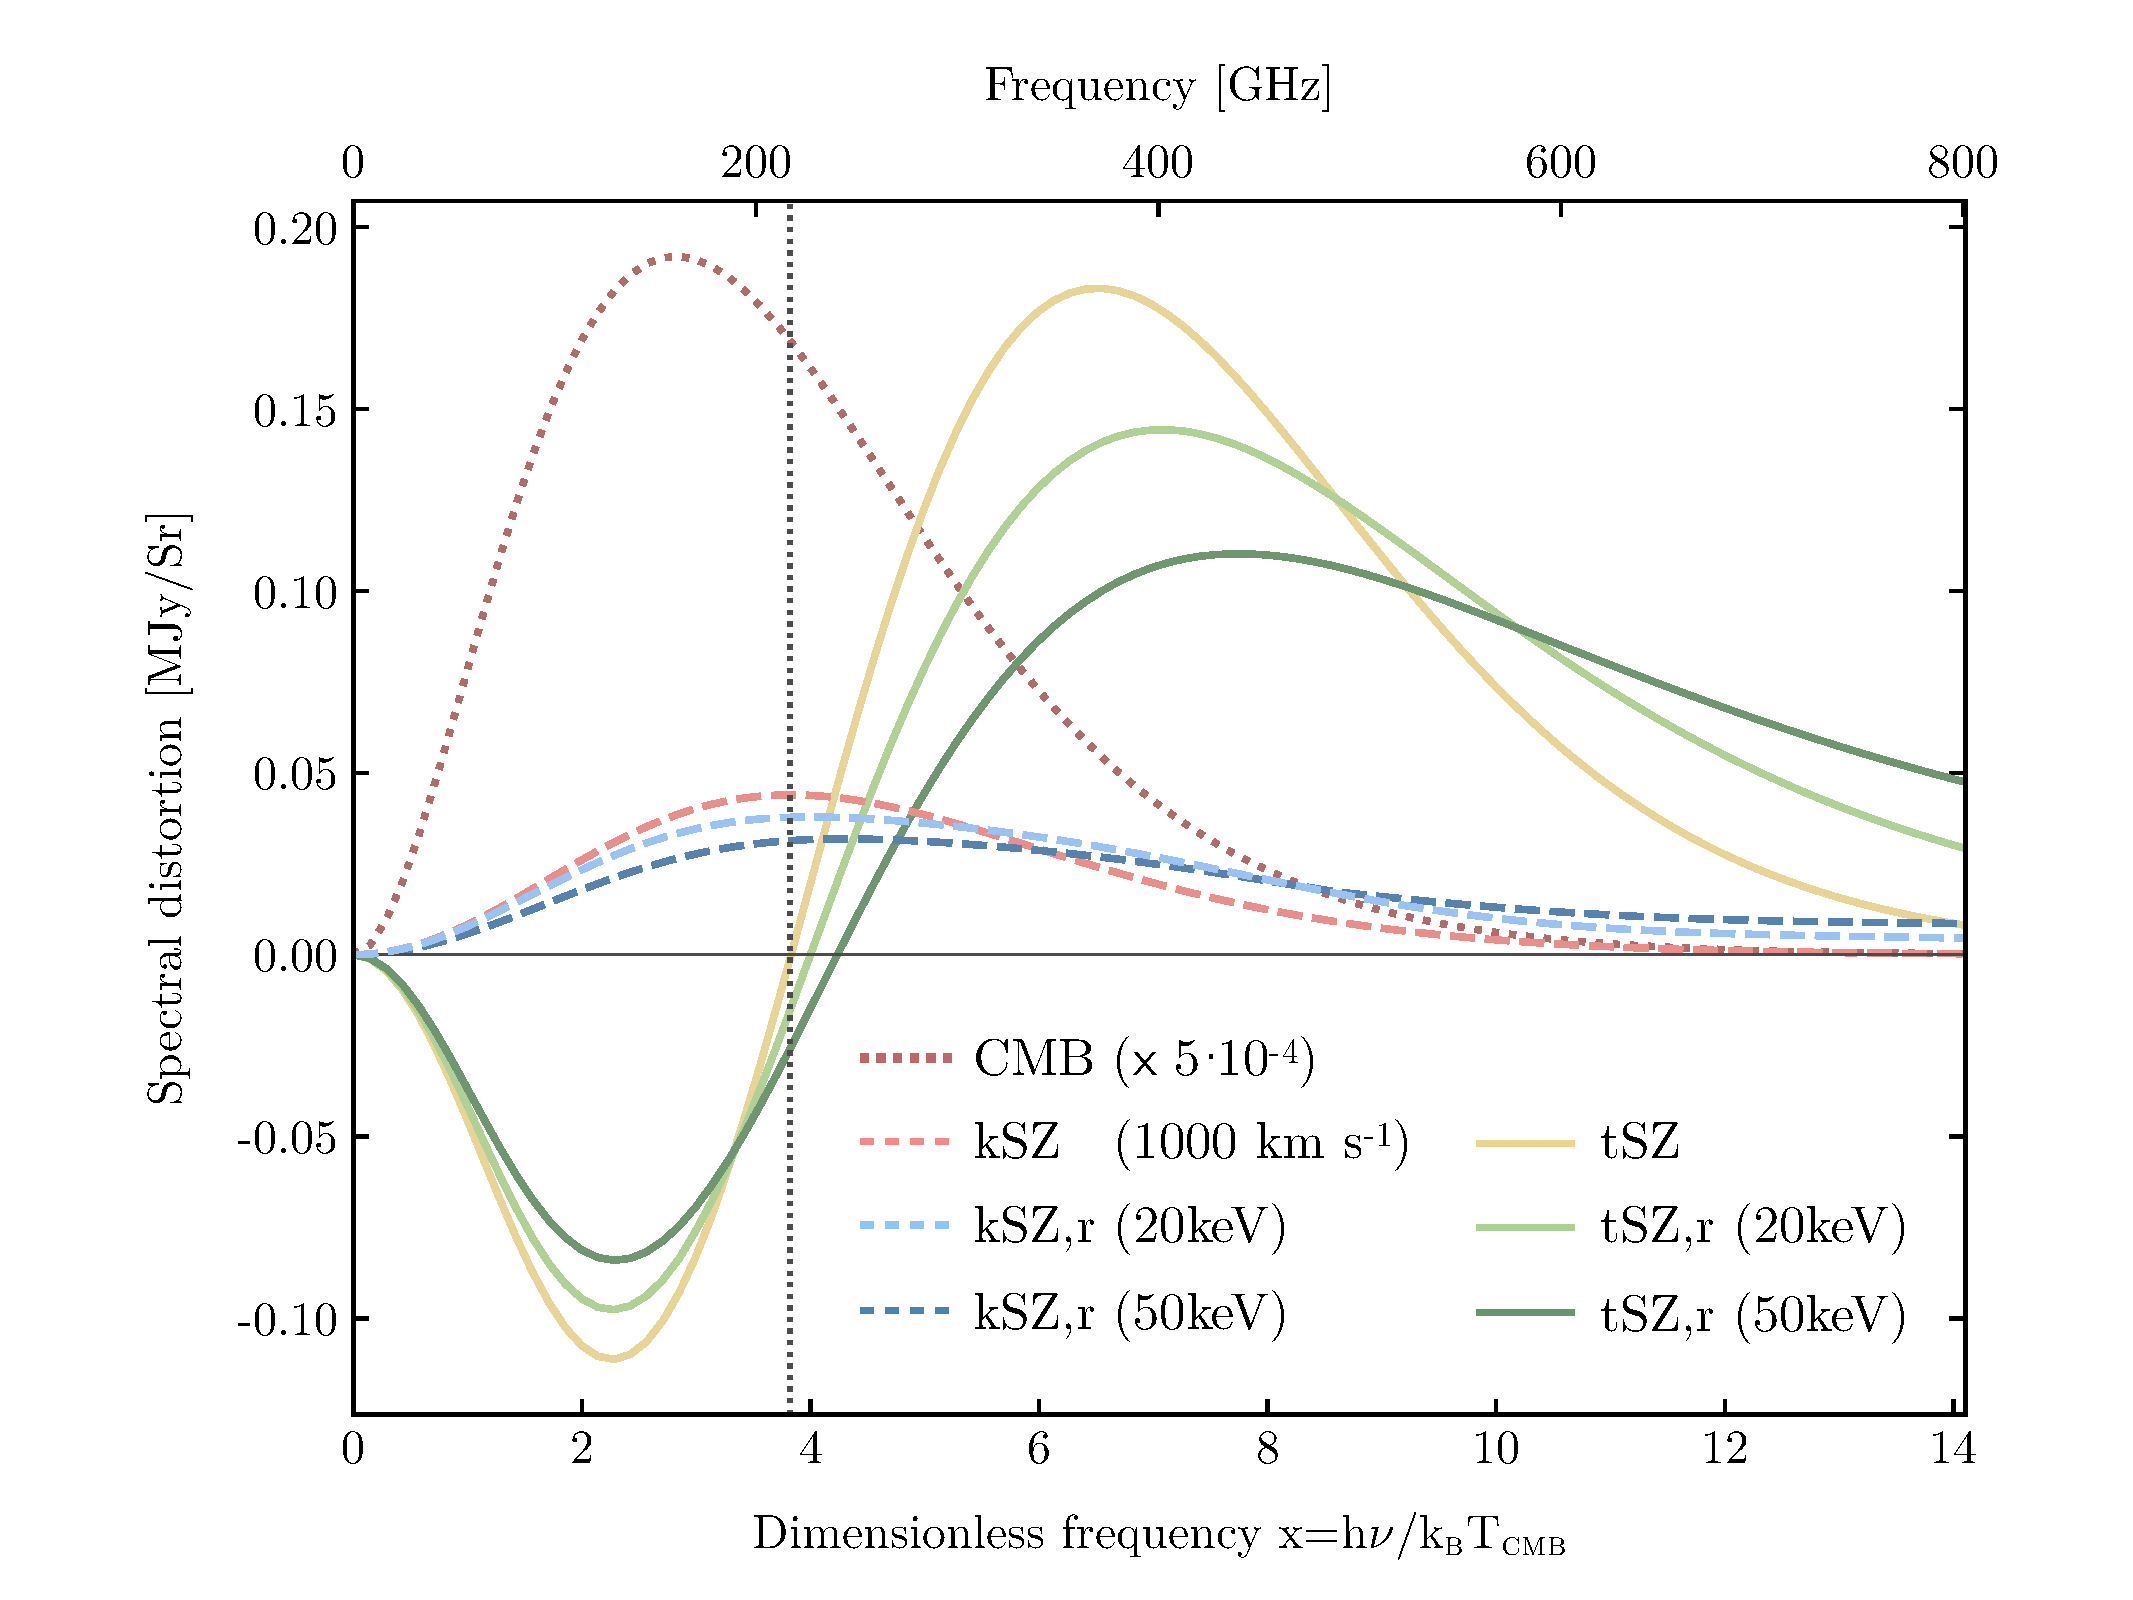
\includegraphics[width=.8\linewidth, trim={0cm 0cm 0cm 1cm}, clip]{Figures/Chap_amas/sz_tony.pdf}
    \caption{
        Spectres de l'effet tSZ (courbes pleines) et kSZ (courbes pointillées), incluant les corrections relativistes pour différentes valeurs de température.
        La profondeur optique considérée est de $\tau_\e = 10^{-2}$.
        Le spectre des photons du CMB sans interaction par effet SZ est également représenté en rouge pour comparaison.
        Figure extraite de \cite{mroczkowski_astrophysics_2019}.
    }
    \label{fig:krsz_spec}
\end{figure*}

\subsubsection{L'effet SZ relativiste} % ---------------------------------------------- %
Les corrections relativistes aux effets tSZ et kSZ, apparaissant respectivement dans les équations (\ref{eq:sz_dI}) et (\ref{eq:ksz_y}), sont parfois regroupées sous le terme d'effet SZ relativiste, ou effet rSZ.
La raison de cette dénomination est la signature spectrale particulière de ces corrections relativistes, permettant de les différencier des contributions au premier ordre des effets tSZ et kSZ, ainsi que le fait qu'elles encodent une information sur les propriétés du milieu intra-amas différentes de ces derniers.
Il est toutefois à noter qu'il s'agit bel et bien seulement de corrections relativistes aux effets susmentionnés: l'effet rSZ ne peut être détecté seul sans la présence des effets principaux.

Nous avons jusqu'à présent négligé les corrections relativistes aux effets SZ.
Cette hypothèse est facilement vérifiée dans le cas de l'effet kSZ, où les mouvements d'ensemble du milieu intra-amas ont des vitesses de l'ordre de la centaine de kilomètres par seconde, soit $\beta = v/c \sim 10^{-4}$.
Elle est moins évidente dans le cas de l'effet tSZ, où une température de $k_\textsc{b} T_\e \sim 1-10 \;{\rm keV}$ conduit à des vitesses\footnotemark $\beta = \sqrt{3 k_\textsc{b} T_\e / 2 m_\e c^2} \sim 0.1$.
\footnotetext{D'après la théorie des gaz parfaits.}

Le calcul des corrections relativistes ne sera pas détaillé ici, et nous renvoyons le lecteur vers des revues telles que \cite{mroczkowski_astrophysics_2019} pour plus de détails.
En pratique, l'effet rSZ dépend principalement de la température du milieu intra-amas, et a pour conséquence l'étalement des spectres des effets tSZ et kSZ, ainsi que le décalage de la fréquence à laquelle la distorsion due à l'effet tSZ s'annule.
Ces effets sont illustrés sur la figure \ref{fig:krsz_spec}: pour des températures croissantes, les amplitudes des spectres tSZ et kSZ sont diminuées aux fréquences inférieures à $\sim 400 \;{\rm GHz}$, et augmentées au-delà.
La fréquence correspondant au zéro de l'effet tSZ est également augmentée, de $217 \;{\rm GHz}$ en négligeant les corrections relativistes, à $\sim 240 \;{\rm GHz}$ pour une température de $k_\textsc{b} T_\e = 50 \;{\rm keV}$.
D'un point de vue observationnel, l'effet rSZ induit donc une modification des signaux tSZ et kSZ dépendant de la température du milieu intra-amas.
Cette modification peut être détectée en observant les effets SZ en provenance d'amas à un grand nombre de fréquences, afin de pouvoir séparer les contributions des termes thermique, cinétique et relativiste.
L'effet rSZ n'a à ce jour été détecté que dans des analyses sur l'empilement du signal SZ de plusieurs amas (\eg\ \cite{hurier_high_2016}), ou à travers son impact sur le spectre de puissance de la cartographie de l'effet SZ sur tout le ciel (\eg\ \cite{remazeilles_can_2019}).
Des études sont en cours pour essayer d'en obtenir des mesures individuelles, qui permettraient une première mesure de la température du milieu intra-amas aux longueurs d'ondes millimétriques, par exemple avec le spectromètre CONCERTO \cite{the_concerto_collaboration_wide_2020}.

D'autres composantes de l'effet Sunyaev-Zeldovich existent, telles que l'effet SZ polarisé ou non-thermique.
Cette thèse étudie exclusivement la composante thermique; toute mention ultérieure de l'effet SZ fera référence à l'effet tSZ, à moins que le contraire soit explicitement écrit.

% ------------------------------------------------------------------------------------- %
\subsection{Relevés d'amas de galaxies par effet SZ}

Comme nous le verrons dans la section \ref{sec:cluster_nbcount}, la contrainte des paramètres cosmologiques à l'aide d'amas de galaxies requiert la connaissance d'un catalogue d'amas de masses et redshifts connus.
De tels catalogues peuvent être construits à partir d'observations de grandes portions du ciel dans l'une des longueurs d'onde auxquelles les amas de galaxies sont détectables, puis par recensement des amas présents dans ce champ.

\subsubsection{Détection par filtre adapté} % ----------------------------------------- %
Dans le cas de l'effet SZ, la détection des amas est faite à partir de cartes dans le domaine millimétrique.
Les algorithmes de détection d'amas utilisés sont basés sur des techniques de filtre adaptés (\textit{matched filter}, voir par exemple \cite{melin_catalog_2006, melin_comparison_2012, zubeldia_understanding_2021}).
Cette approche consiste en l'exploitation d'une connaissance \prior\ de la distribution attendue du signal typique d'un amas de galaxies, et de la dépendance spectrale de l'effet étudié.
Considérons un relevé du ciel à plusieurs fréquences du domaine millimétrique $\nu_i, \, i \in [1 \dots N]$, comme le relevé réalisé à l'aide de l'instrument HFI du satellite \textit{Planck} \cite{lamarre_planck_2010,planck_collaboration_planck_2020-1}.
Les cartes peuvent être regroupées dans un vecteur $\mathbf{M}$, dont la composante $i$ représente la carte à la fréquence $\nu_i$:
\begin{equation}
    \label{eq:matched_filter}
    \mathbf{M}(\vec{x}) = y_0 \, \mathbf{S}(\vec{x}, \theta_c) + \mathbf{N}(\vec{x}),
\end{equation}
où $\vec{x}$ représente les coordonnées célestes observées, $y_0$ le paramètre de Compton central d'un amas, $\mathbf{S}(\vec{x}, \theta_c)$ la distribution spatiale du signal SZ d'un amas de taille $\theta_c$, et $\mathbf{N}(\vec{x})$ un vecteur analogue à $\mathbf{M}$ contenant les cartes de bruit aux différentes fréquences, incluant le bruit instrumental et astrophysique. \\
On définit alors un filtre adapté $\mathbf{\psi}(x, \theta_c)$, dont la transformée de Fourier s'écrit:
\begin{equation}
    \label{eq:matched_filter_filter}
    \mathbf{\psi}(\vec{k}, \theta_c) = \mathbf{\sigma}^2(\theta_c) \, \mathbf{P}^{-1}(\vec{k}) \, \mathbf{S}(\vec{k}, \theta_c),
\end{equation}
où $\mathbf{\sigma}^2(\theta_c)$ est la variance dans la carte de bruit convoluée par le filtre considéré, et $\mathbf{P}(\vec{k})$ le spectre de puissance de la carte de bruit $\mathbf{N}$. \\
La convolution des cartes formant le vecteur $\mathbf{M}$ par ce filtre permet alors d'obtenir un estimateur non-biaisé du paramètre de Compton central des amas,
\begin{equation}
    \hat{y}_0 = \int \mathbf{\psi}(\vec{x}, \theta_c) \, \mathbf{M}(\vec{x}) \, \d\vec{x}.
\end{equation}
La procédure est répétée pour plusieurs valeurs de taille de filtre $\theta_c$, afin de pouvoir détecter aussi bien des amas étendus que compacts.

Les cartes ainsi filtrées permettent d'identifier les positions des pics de paramètre de Compton, correspondant aux positions abritant des amas de galaxies.
La significativité de ces pics, donnée par les cartes du rapport $\hat{y}_0 / \sigma(\theta_c)$, permet d'associer à chaque pic la probabilité qu'il soit effectivement lié à un amas.
Ainsi, seuls les détections de significativité supérieure à un seuil fixé sont considérées comme des détections.
Le choix de ce seuil reflète la nécessité d'un compromis entre la pureté (fraction de faux positifs, détections non associées à un amas de galaxies) et la complétude (fractions d'amas existants effectivement détectés, liée au taux de faux négatifs).
En effet, plus le seuil sera bas, plus un catalogue sera complet (car incluant les amas de faible significativité), mais moins il sera pur (car composé de plus de détections ne correspondant pas à des amas).

\subsubsection{Profil de pression moyen des amas} % ----------------------------------- %
\label{sec:univ_press_prof}
Les cartes composant les vecteurs $\mathbf{M}$ et $\mathbf{N}$ dans l'équation (\ref{eq:matched_filter}) étant connues\footnotemark, l'enjeu est l'utilisation du meilleur modèle possible pour la distribution radiale du signal de l'amas, $\mathbf{S}$.
\footnotetext{Le signal SZ étant largement sous-dominant dans les relevés du ciel par rapport aux signaux contaminants (comme l'atmosphère) ou astrophysiques (comme les anisotropies primaires du CMB), les spectres de puissance des cartes de bruit $\mathbf{N}(\vec{x})$ sont en général supposés égaux à ceux des cartes complètes $\mathbf{M}(\vec{x})$.}
En effet, une mauvaise connaissance de la distribution du signal SZ en direction d'un amas entraînera de mauvaises performances pour l'algorithme de détection.

Du fait du lien entre l'amplitude de l'effet tSZ et la pression du milieu intra-amas (équation \ref{eq:sz_y}), la connaissance de la distribution radiale du signal requiert une connaissance \prior\ du profil de pression des amas\footnotemark.
\footnotetext{On note qu'il est également possible de s'affranchir de cette connaissance en utilisant un filtre adapté modélisant directement le profil de paramètre de Compton $y$, par exemple avec un smple modèle $\beta$ (approche utilisée par exemple dans les relevés réalisés à partir des données SPT, \eg\ \cite{bleem_sptpol_2020}).}
En effet, connaître la distribution de pression dans le milieu intra-amas permet d'estimer la distribution de paramètre de Compton par intégration le long de la ligne de visée, et donc la distribution de brillance de surface de l'effet tSZ.
La connaissance du profil de pression tridimensionnel moyen des amas $P(r)$ permet donc de remonter à un profil de paramètre de Compton dans le ciel $y(\vec{x})$.
Celui-ci peut alors être utilisé pour calculer le modèle de distribution spatiale de signal SZ nécessaire au calcul du filtre adapté (équation \ref{eq:matched_filter_filter}):
\begin{equation}
    \label{}
    \mathbf{S}(\vec{x}, \theta_c) = f(\nu_i) \left[ b_i \ast y(\vec{x}, \theta_c) \right],
\end{equation}
où $f(\nu)$ est la dépendance spectrale de l'effet SZ (équation \ref{eq:sz_dI}), et $b_i$ le lobe\footnotemark\ de l'instrument utilisé pour réaliser les mesures à la fréquence $\nu_i$.
\footnotetext{Le \guillemotleft lobe \guillemotright\ d'un instrument est le terme employé en radioastronomie pour désigner sa fonction d'étalement du point, ou PSF pour \textit{point spread function}.}

De plus, les cartes obtenues par convolution par le filtre adapté permettent la mesure du paramètre de Compton intégré par intégration polaire du profil de paramètre de Compton.
Par exemple, dans un rayon caractéristique $R_{500}$, on a
\begin{equation}
    \label{eq:sz_yinteg_cyl}
    Y_{500}^{\rm cyl.} = 2\pi \int_0^{\theta_{500}} \hat{y}(\theta) \theta \, \d\theta,
\end{equation}
où $\theta_{500} = c_{500} \, \theta_c$ est l'angle sous-tendu par le rayon caractéristique $R_{500}$, avec $c_{500}$ le paramètre de concentration de l'amas. \\
On note une différence fondamentale entre les grandeurs $Y_{500}$ et $Y_{500}^{\rm cyl.}$ définis dans les équations (\ref{eq:sz_yinteg}) et (\ref{eq:sz_yinteg_cyl}).
Dans la première, l'intégration réalisée est celle du profil de pression dans une sphère de rayon $R_{500}$, alors que la seconde revient à une intégration dans un cylindre de rayon $R_{500}$ et de profondeur infinie.
En pratique, la différence est faible, puisque la pression au-delà de $R_{500}$ est plusieurs ordres de grandeur plus faible qu'à l'intérieur de ce rayon.
Pour le profil de pression universel des amas de galaxies mesuré par \myciteauthor{arnaud_universal_2010} (discuté au paragraphe suivant), le rapport entre les deux est de $0.83$ (voir section 6 de \cite{arnaud_universal_2010}).
Dans la suite, nous considèrerons des valeurs calculées par intégration sphérique.

Le profil de pression moyen du milieu intra-amas est donc l'un des ingrédients nécessaires aux études cosmologiques basées sur l'effet SZ.
Dans l'hypothèse autosimilaire, la distribution radiale des propriétés thermodynamiques du milieu intra-amas doit pouvoir être bien décrite par un profil universel, mis à l'échelle par rapport à leur masse et taille caractéristique.
Les écarts à cette hypothèse proviennent de la diversité des phénomènes physiques liés aux baryons et pouvant modifier le contenu énergétique des amas.
Le profil de pression, étant directement lié au potentiel gravitationnel de l'amas par l'équation de Poisson, est supposé être le moins affecté par ces phénomènes, et particulièrement bien décrit par un profil moyen à l'échelle.
Cette hypothèse a été vérifiée expérimentalement à plusieurs reprises, menant à plusieurs mesures du profil de pression dit universel des amas de galaxies.
L'exemple le plus notable est le profil universel de \myciteauthor{arnaud_universal_2010}, mesurant le profil de pression moyen de 33 amas de galaxies à bas redshift ($z < 0.2$), en utilisant des observations X seulement.
Le profil résultant est représenté en figure \ref{fig:a10_upp}.
Cette étude montre que le profil de pression des amas est remarquablement autosimilaire: les profils des différents amas normalisés par leur masse (courbes noires en \ref{fig:a10_upp}) montrent très peu de dispersion.
Cela atteste du fait que les amas se comportent bien comme des répliques à l'échelle les uns des autres.

\begin{figure*}[t]
    \centering
    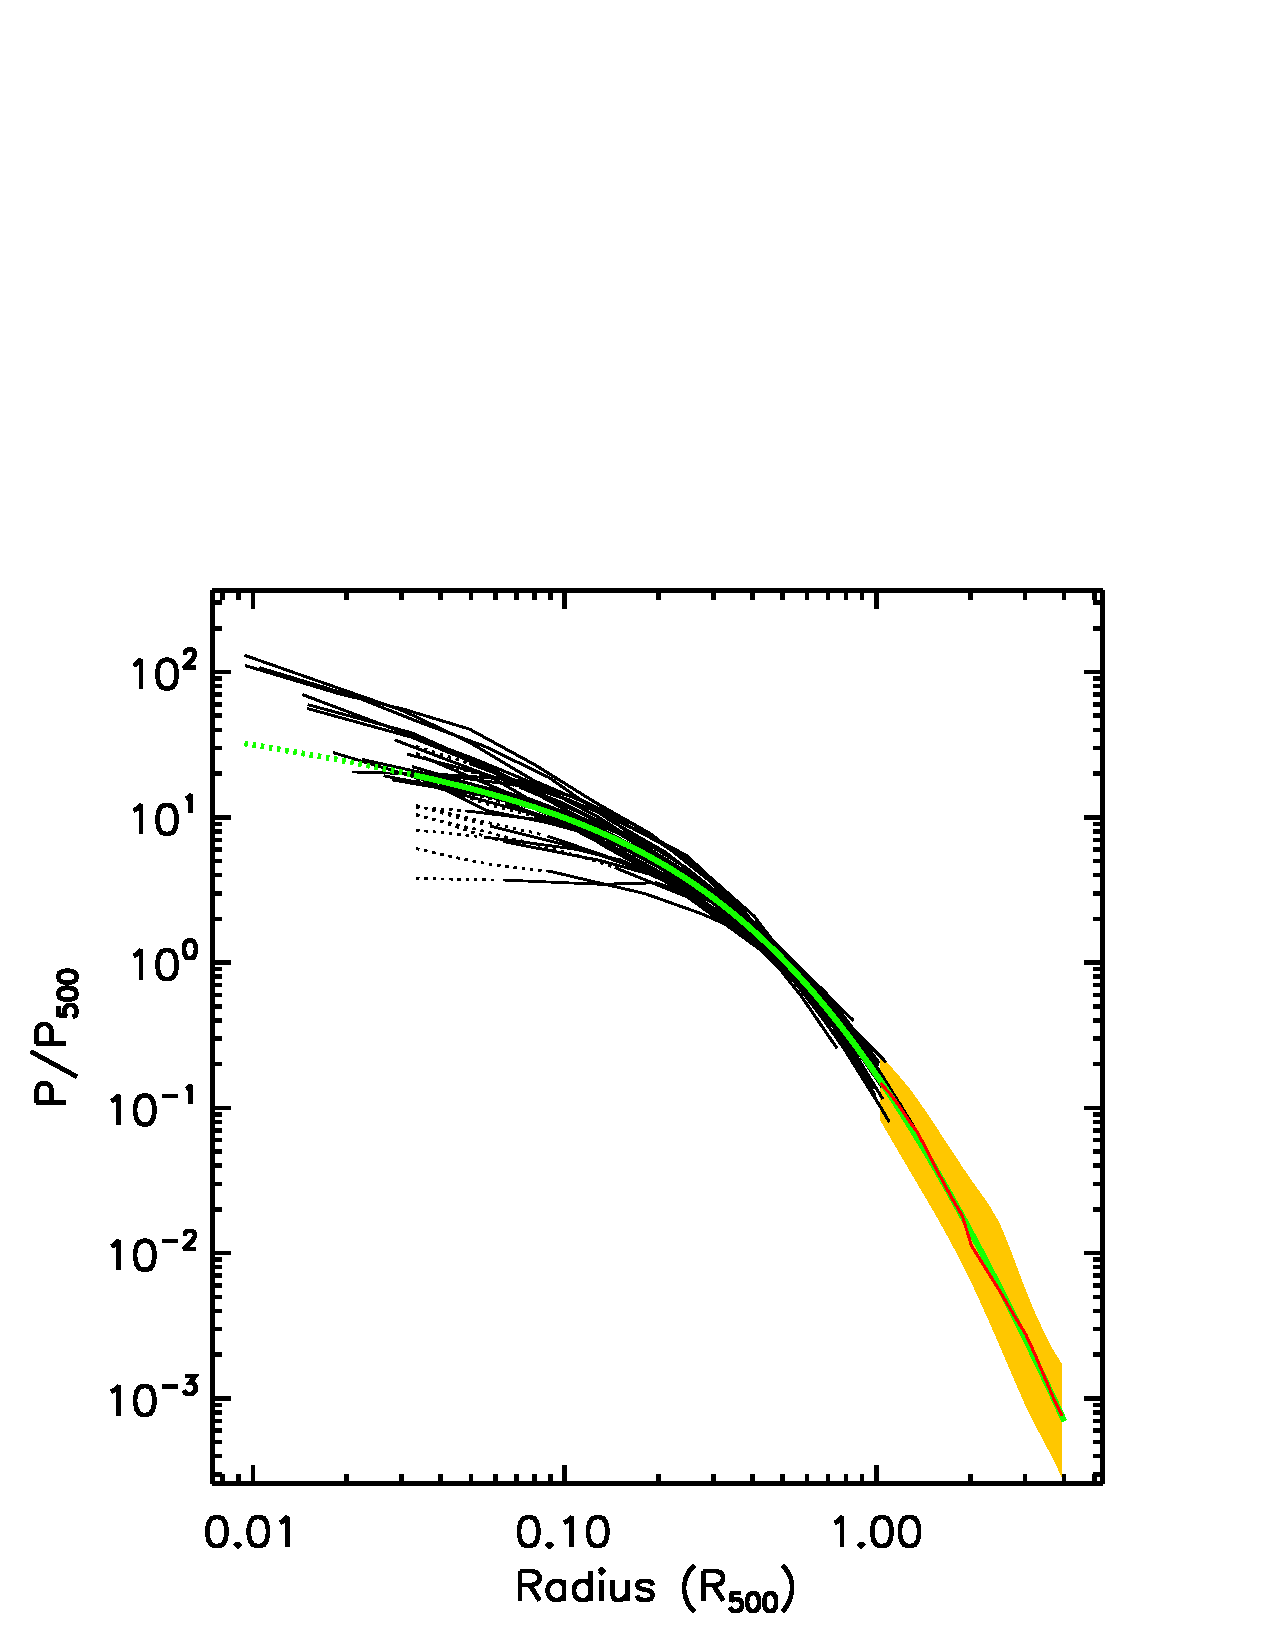
\includegraphics[width=.6\linewidth]{Figures/Chap_nk/Fig_universal.pdf}
    \caption{
        Profils de pression des amas de galaxies de l'échantillon REXCESS mesurés par \textit{XMM-Newton} (noir) et profil de pression moyen de l'échantillon, dit universel (vert).
        Figure extraite de \cite{arnaud_universal_2010}.
    }
    \label{fig:a10_upp}
\end{figure*}

% ===================================================================================== %
\section{Cosmologie par comptage d'amas de galaxies} \label{sec:cluster_nbcount}

Le lien étroit entre la formation et l'évolution des amas de galaxies et la cosmologie fait de ces derniers d'excellents outils pour la mesure des propriétés de l'Univers (voir par exemple \cite{allen_cosmological_2011} pour une revue).
Ce lien peut être exploité de plusieurs façons complémentaires, du diagramme de Hubble des amas (\eg\ \cite{kozmanyan_deriving_2019}) au spectre de puissance de l'effet SZ (\eg\ \cite{ruppin_impact_2019}), en passant par la fraction de gaz dans les amas (\eg\ \cite{mantz_cosmology_2014}).
Dans cette thèse, nous sous intéresserons au comptage d'amas de galaxies par intervalles de masse et de redshift.
Cette section présente le principe des contraintes cosmologiques par comptage d'amas.

% ------------------------------------------------------------------------------------- %
\subsection{Fonction de masse et comptage d'amas}

Comme décrit dans la section \ref{sec:cosmo_hmf}, la fonction de masse $\d N / \d M$ quantifie le nombre de halos par unité de masse dans l'Univers (équation \ref{eq:hmf}).
Afin de pouvoir l'utiliser pour prédire un nombre d'amas visibles par un observateur, il est nécessaire de tenir compte du fait que seule une portion limitée de l'Univers lui est accessible.
Deux raisons motivent ce constat.
Premièrement, l'angle solide $\Omega$ couvert par des observations doit être pris en compte, puisque les amas situés en dehors de cette région ne pourront pas être détectés.
Deuxièmement, il est nécessaire de calculer le volume effectivement accessible à un redshift donné.
Étant donné la vitesse de déplacement finie de la lumière, celle qui nous parvient depuis un amas a été émise à une époque ancienne, à un redshift d'autant plus grand que l'amas est distant.
Le volume accessible dans une tranche de redshifts $z_1 < z < z_2$ est donc celui d'une coquille sphérique, de volume
\begin{equation}
    V_c = \frac{4\pi}{3}\left[\chi^3(z_2) - \chi^3(z_1)\right],
\end{equation}
où $\chi(z)$ est la distance comobile entre l'observateur et un point de redshift $z$, qui dépend des paramètres cosmologiques. \\
On définit alors l'abondance d'amas par unités de masse, de redshift et d'angle solide potentiellement accessibles par un observateur comme:
\begin{equation}
    \label{eq:hmf_comoving}
    \frac{\d N}{\d M \, \d z \, \d\Omega} = \frac{\d N}{\d M} \frac{\d V_c}{\d z \, \d\Omega}.
\end{equation}
Enfin, la complétude du relevé traduit la probabilité de détecter un amas de galaxies à une masse $M$, un redshift $z$ et une position $\vec{r}$ donnée.
Cette probabilité est nommée \textit{fonction de sélection en masse} du relevé, $\hat{\chi}(z, M; \vec{r})$, et dépend à la fois de l'éventuelle anisotropie de la couverture du ciel réalisée, mais également de l'observable des amas considérée et de l'algorithme utilisé pour leur détection, comme discuté dans la section \ref{sec:scaling}.

Le nombre d'amas potentiellement observables entre des redshifts $z_1$ et $z_2$, entre des masses $M_1$ et $M_2$, pour un relevé de complétude $\hat{\chi}$ couvrant un angle solide $\Omega$, est alors donné par:
\begin{equation}
    \label{eq:nbcount_mass}
    n(\vec{\vartheta}) %(z_1 \leqslant z \leqslant z_2, M_1 \leqslant M \leqslant M_2)
    = \int_{z_1}^{z_2} \d z
      \int_\Omega \d\Omega'
      \int_{M_1}^{M_2} \d M \,
        \hat{\chi}(z, M; \Omega') \frac{\d N}{\d M} \frac{\d V_c}{\d z \, \d\Omega'}.
\end{equation}
Celui-ci dépend des paramètres cosmologiques $\vec{\vartheta}$ au travers de la fonction de masse $\d N / \d M$ et du volume comobile $V_c$.
Ainsi, un catalogue d'amas de masses et redshifts connus peut être organisé en différentes classes $i$ de masse et redshift, et le nombre d'amas dans chaque classe $N_i$ peut être comparé à celui attendu pour un jeu de paramètres cosmologiques $\vec{\vartheta}$.
Les nombres d'amas dans chaque classe représentant un comptage discret, la comparaison se fait par le biais d'une fonction de vraisemblance poissonienne:
\begin{equation}
    \label{eq:nbcount_likelihood}
    {\rm ln}\, \mathcal{L}
    = \sum_i {\rm ln}\, P(N_i \,|\, \vec{\vartheta})
    = \sum_i \left[N_i \; {\rm ln}\, n_i(\vec{\vartheta}) - n_i(\vec{\vartheta}) - {\rm ln}\, N_i! \right].
\end{equation}
Cette fonction de vraisemblance peut être utilisée pour chercher le jeu de paramètres cosmologiques générant les comptages d'amas décrivant le mieux le jeu de données observé, ou encore injecté dans une procédure Monte Carlo à Chaînes de Markov (MCMC) pour trouver les distributions de probabilité permises pour les paramètres cosmologiques.
De telles analyses seront détaillées dans le cadre de l'analyse des propriétés thermodynamiques du milieu intra-amas, au chapitre \ref{chap:panco}.
L'exploitation cosmologique d'un relevé d'amas de galaxies requiert donc l'obtention d'un catalogue d'amas dont la masse et le redshift sont connus, qui peut être comparé à un modèle dépendant des paramètres cosmologiques à travers l'équation (\ref{eq:nbcount_likelihood}).

Un exemple d'analyse par comptage d'amas et de ses résultats est présenté en figure \ref{fig:nbcount_bocquet}, illustrant la distribution d'amas en redshift dans l'échantillon SPT-SZ $2500 \;{\rm deg^2}$ \cite{bleem_galaxy_2015} et les résultats cosmologiques issus de l'analyse \cite{bocquet_cluster_2019}.
On observe sur le panneau droit l'histogramme du nombre d'amas détectés par classes de redshift (en bleu) dans le relevé.
La région verte montre les intervalles de confiance de l'ajustement de cet histogramme par un modèle de comptage d'amas (équation \ref{eq:nbcount_mass}), en utilisant une fonction de vraisemblance similaire à l'équation (\ref{eq:nbcount_likelihood}).
Les paramètres ajustés sont (entre autres) les paramètres cosmologiques $\Omega_m$ et $\sigma_8$ d'un modèle cosmologique standard $\Lambda{\rm CDM}$.
Le panneau droit montre les intervalles de confiance obtenus sur ces deux paramètres en bleu.
Des études similaires ont pu être menées à partir des relevés réalisés par les instruments \textit{Planck} \cite{planck_collaboration_planck_2016-2} et ACT \cite{hilton_atacama_2021}.

\begin{figure*}[t]
    \centering
    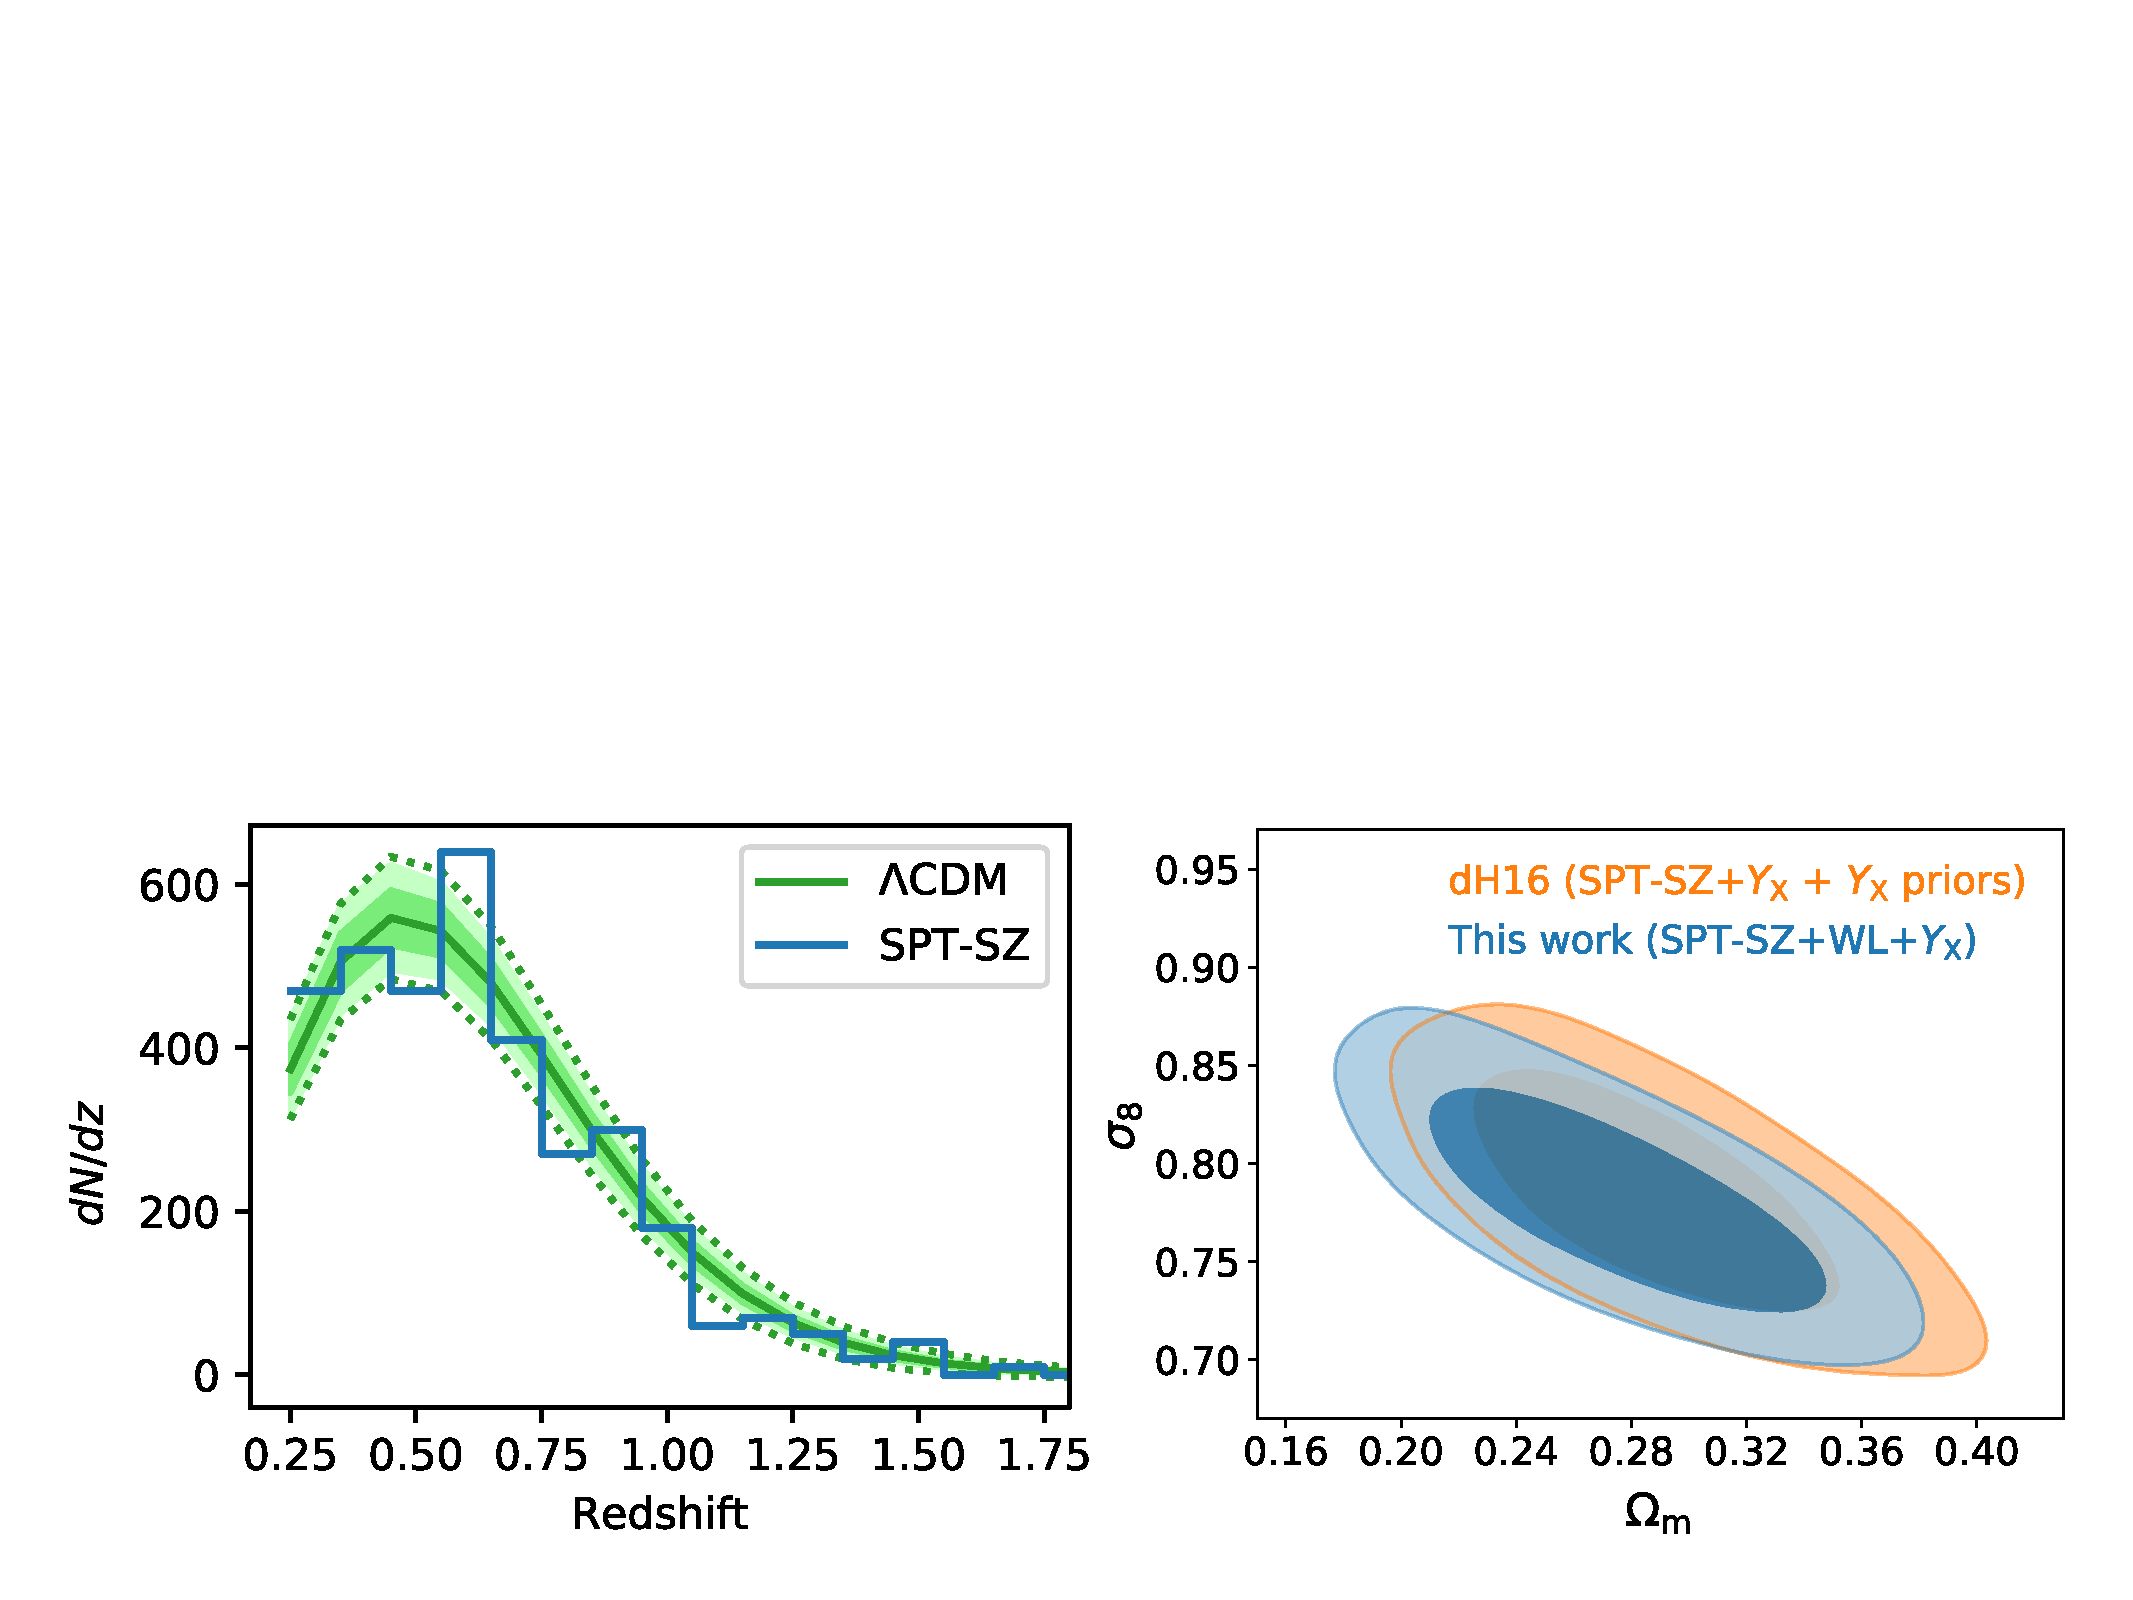
\includegraphics[width=\linewidth]{Figures/Chap_amas/bocquet.pdf}
    \caption{
        \textbf{Gauche:} Comptage d'amas par intervalles de redshift dans le relevé SPT-SZ $2500 \;{\rm deg^2}$ (bleu) et résultats de l'ajustement du modèle de l'équation (\ref{eq:nbcount_mass}) (vert).
        \textbf{Droite:} Intervalles de confiance à $1\sigma$ et $2\sigma$ obtenus sur les paramètres $(\Omega_m, \sigma_8)$ par l'ajustement représenté dans le panneau gauche (bleu).
        L'ellipse orange montre les résultats de l'étude antérieure de \cite{de_haan_cosmological_2016} pour comparaison.
        Figures adaptées de \cite{bocquet_cluster_2019}.
    }
    \label{fig:nbcount_bocquet}
\end{figure*}

% ------------------------------------------------------------------------------------- %
\subsection{Relation d'échelle masse-observable}\label{sec:scaling}

Nous avons vu dans la section précédente que les analyses cosmologiques nécessitaient l'obtention d'un catalogue d'amas de galaxies et la connaissance de leurs masses.
Il s'agit d'une contrainte forte: en pratique, peu de relevés d'amas sont en mesure d'accéder aux valeurs des masses individuelles des amas qu'ils détectent.
Il est donc nécessaire pour chaque relevé de quantifier le lien entre la masse des amas et l'une des observables directes du catalogue.
Ce lien est nommé relation d'échelle masse-observable, et sa connaissance est cruciale afin de pouvoir mener des analyses cosmologiques précises et justes.
Le chapitre \ref{chap:scaling} sera entièrement consacré à l'étude de cette relation d'échelle dans le cas de relevés SZ.
Nous nous restreindrons donc ici aux éléments essentiels pour comprendre la nécessité de telles relation pour la cosmologie avec des amas.

Les relations d'échelle fournissent donc une estimation de la masse d'un amas à partir d'une grandeur observable d'un relevé.
L'observable considérée doit donc être étroitement liée à la masse pour des contraintes précises: on qualifie alors l'observable de \textit{proxy} de masse.
Parmi les observables utilisées, on trouve la significativité de la détection des amas, c'est-à-dire la probabilité qu'une détection corresponde à un amas.
Cette grandeur est un résultat direct de beaucoup d'algorithmes de détection d'amas dans toutes les longueurs d'onde, et est fréquemment utilisée comme \textit{proxy} de masse dans les analyses cosmologiques\footnote{Par exemple dans les analyses des données SPT en SZ \cite{bocquet_cluster_2019} utilisées à titre d'exemple dans la section \ref{sec:cluster_nbcount}.}.
Plusieurs autres observables peuvent être considérées selon la longueur d'onde considérée.
En X, la luminosité et la température du milieu intra-amas sont souvent utilisées (\eg\ \cite{pacaud_xxl_2018}).
En optique, comme évoqué dans la section \ref{sec:opt}, la richesse des amas, définie par le nombre de galaxies membres, est fréquemment utilisée (\eg\ \cite{des_collaboration_dark_2020}).
En SZ, le paramètre de Compton intégré $Y_\Delta$, quantifiant le contenu en énergie thermique dans le milieu intra-amas (cf équation \ref{eq:sz_yinteg}), est fréquemment employé, pour des valeurs de contraste $\Delta$ dépendant de la couverture angulaire de l'instrument utilisé.

L'étalonnage de la relation d'échelle est effectuée en étudiant le lien entre masse des amas et observables pour un échantillon d'amas de masses connues.
Un tel échantillon peut être dressé de deux façons.
Dans le cas où un relevé offre une mesure directe de masse pour certains amas, la relation d'échelle peut être calculée à partir de ceux-ci: on parle alors d'auto-étalonnage.
Par exemple, dans un relevé optique (cf. section \ref{sec:opt}), une fraction d'amas peut avoir des masses mesurées par lentillage gravitationnel; la relation entre leur richesse et cette masse est alors calculée, et appliqué à tous les amas dont les galaxies d'arrière-plan ne permettent pas une mesure de masse (\eg\ \cite{andreon_richness-mass_2012}).
De même, les amas émettant fortement en X pourront permettre une mesure de masse par combinaison de leurs profils de densité et de température obtenu par spectroscopie (cf. section \ref{sec:x}).
Dans le cas où un relevé ne permet pas de mesure directe, une mesure de masse peut être obtenue par combinaison avec des données issues d'autres relevés, ou bien par un suivi dédié d'un échantillon d'amas.
Les bénéfices apportés par de tels suivis seront discutés en \ref{sec:follow_ups}.
Dans les deux cas, il est important que l'échantillon d'amas dont les masses sont connues soit représentatif de la population sous-jacente, afin d'éviter de biaiser les analyses par l'étude d'une population d'amas aux propriétés particulières.

Les relations d'échelle sont le plus souvent modélisées comme une relation en loi de puissance entre l'observable et la masse.
Alors, l'étude de la relation entre les logarithmes de l'observable et de la masse devient une relation affine:
\begin{equation}
    \label{eq:scaling_noproba}
    \log Y = \alpha_\ym + \beta_\ym \log M.
\end{equation}
Dans une approche probabiliste, la relation d'échelle peut être interprétée comme la probabilité pour un amas de masse $M$ d'être détecté avec une valeur d'observable $Y$.
Cette approche permet de tenir compte de la dispersion intrinsèque autour de la relation d'échelle: en effet, les différents phénomènes physiques ayant lieu au sein d'un amas peuvent affecter les observables sans modifier la masse.
En modélisant cette dispersion comme gaussienne, la relation d'échelle peut s'écrire:
\begin{equation}
    \label{eq:scaling_pdf}
    P(\log Y \,|\, \log M) = \N(\alpha_\ym + \beta_\ym \log M, \sigma_{\rm int}^2)
\end{equation}
où $\N(\mu, v)$ est la distribution de probabilité d'une loi normale de moyenne $\mu$ et de variance $v$, et $\sigma_{\rm int}$ est la dispersion intrinsèque de la relation.

L'ajustement des relations d'échelle est complexe, et peut être faire appel à un grand nombre de méthodes selon les objectifs (voir par exemple la revue de \cite{andreon_measurement_2013}).
Le chapitre \ref{chap:scaling} de cette thèse sera consacré à de tels ajustements dans le cadre d'un modèle bayésien hiérarchique.
Une fois connue, la relation d'échelle peut être injectée dans l'équation (\ref{eq:nbcount_mass}) pour exprimer cette dernière en termes d'observables plutôt que de masse.
Le nombre d'amas potentiellement observables entre des redshifts $z_1$ et $z_2$, entre des valeurs d'observable $Y_1$ et $Y_2$ est alors donné par:
\begin{equation}
    \label{eq:nbcount_obs}
    n(\vec{\vartheta}, \vec{\vartheta}')
    = \int_{z_1}^{z_2} \d z
      \int_\Omega \d\Omega'
      \int \d M \,
      \int_{Y_1}^{Y_2} \d Y \,
        \chi(z, Y; \Omega') \frac{\d N}{\d M} \frac{\d V_c}{\d z \, \d\Omega'}.
\end{equation}
où $\chi(z, Y; \Omega)$ est la \textit{fonction de sélection en observable} du relevé, liée à la fonction de sélection en masse par:
\begin{equation}
    \label{eq:nbcount_sel}
    \hat{\chi}(z, M ; \Omega) = \int P(Y \,|\, M) \chi(z, Y ; \Omega) \, \d Y.
\end{equation}

Le nombre d'amas attendu dépend donc à la fois des paramètres cosmologiques $\vec{\vartheta}$ et des paramètres de la relation d'échelle, $\vec{\vartheta}'$.
La connaissance des valeurs des paramètres $\vec{\vartheta}' = (\alpha_\ym, \beta_\ym, \sigma_{\rm int})$ décrivant le mieux les données est alors insuffisante, puisqu'elle ne permet pas de propager l'incertitude sur ces grandeurs au calcul des paramètres cosmologiques.
Il est donc nécessaire de connaître les distributions de probabilité des paramètres de la relation d'échelle.
Ces distributions peuvent être obtenues par l'ajustement de la relation par MCMC, qui sera discuté dans le chapitre \ref{chap:scaling}, et utilisées comme \prior\ sur les paramètres dans l'ajustement simultané des paramètres cosmologiques et de ceux de la relation d'échelle.
De telles études permettent de tenir compte des effets systématiques associés à l'étalonnage de masse des amas de galaxies dans les analyses cosmologiques (par exemple en SZ \cite{bocquet_cluster_2019} ou en optique \cite{des_collaboration_dark_2020}).

% ===================================================================================== %
\section{État de l'art et perspectives}

% ------------------------------------------------------------------------------------- %
\subsection{Relevés d'amas et résultats cosmologiques actuels}\label{sec:current_surveys}

Le comptage d'amas de galaxies s'est imposé comme l'une des sondes cosmologiques majeures des dernières années grâce à l'augmentation du nombre d'amas détectés dans les relevés réalisés aux différentes longueurs d'onde discutées en \ref{sec:cluster_obs}.

En optique, les relevés du Sloan Digital Sky Survey (SDSS, \cite{rykoff_redmapper_2014,costanzi_methods_2019}), et plus récemment des Dark Energy Survey (DES, \cite{des_collaboration_dark_2020}) et Kilo-Degree Survey (KiDS, \cite{lesci_amico_2020}), ont permis de construire des catalogues de plusieurs milliers d'amas de galaxies, jusqu'à des redshifts d'environ 0.6.
Ces relevés ont utilisé les mesures de lentillage faible pour l'auto-étalonnage des masses des amas de ces catalogues (voir section \ref{sec:scaling}).

Les catalogues d'amas de galaxies dressés grâce aux différents relevés réalisés par le satellite \textit{ROSAT} (\eg\ RASS \cite{bohringer_northern_2000} ou REFLEX \cite{bohringer_rosat-eso_2004}) ont laissé un héritage conséquent pour l'étude des propriétés des amas de galaxies en X, en particulier de leurs propriétés thermodynamiques et des relations d'échelles liant brillance de surface X et masse d'amas (\eg\ \cite{arnaud_universal_2010, pratt_galaxy_2009,pratt_gas_2010}).
Récemment, les relevés d'amas en X ont consisté en plusieurs relevés profonds concentrés sur de petites régions du ciel.
En particulier, le relevé XXL a permis de construire un catalogue de 356 amas dans une région de $50 \;{\rm deg^2}$ jusqu'à des redshifts d'environ 1 \cite{adami_xxl_2018}.

Les différents relevés du CMB réalisés au cours de la dernière décennie ont permis la construction de grands catalogues d'amas grâce à l'effet SZ, notamment avec le satellite \textit{Planck} \cite{planck_collaboration_planck_2016-1}, le South Pole Telescope (SPT, \cite{bleem_sptpol_2020}) et l'Atacama Cosmology Telescope (ACT, \cite{hilton_atacama_2021}).
Ce dernier constitue l'un des relevés d'amas de galaxies les plus grands et profonds existant à la date de l'écriture de cette thèse, avec plus de 4000 amas jusquà des redshifts d'environ 1.9 \cite{hilton_atacama_2021}.

La distribution en masse et redshift des catalogues d'amas obtenus par l'effet SZ est représentée en figure \ref{fig:cluster_catalogs_mz}.
Celle-ci suit la forme du produit de la fonction de masse et du volume comobile, qui fournit une prédiction du nombre d'amas de masse et redshift donné accessible par un observateur\footnotemark.
\footnotetext{Comme expliqué dans la section \mypageref{sec:cluster_nbcount} (équation \ref{eq:hmf_comoving}).}
On voit que la plupart des amas détectés par ces relevés se situent à des redshifts inférieurs à 1.5, et à des masses supérieures à $2 \times 10^{14} \;M_\odot$.
On y observe également les couvertures en masse et redshift de chacun des relevés.
Le relevé réalisé avec le satellite \textit{Planck} est caractérisé par une moins grande résolution angulaire que ses contreparties au sol, due à la difficulté technique liée à l'envoi d'un télescope aussi large que le SPT (10 m) ou l'ACT (6 m) dans l'espace.
Par conséquent, il est sensible à de plus grandes échelles angulaires, ce qui le rend plus complet à bas redshift et haute masse, mais moins à haut redshift et faible masse.
La profondeur du relevé influe également sur la possibilité de détecter des amas.
Ainsi, les relevés ACT et SPT, plus profonds que le relevé \textit{Planck}, sont plus complets pour les amas peu lumineux (de basse masse) que ce dernier.
Enfin, le nombre d'amas détectés par un relevé dépend évidemment de sa couverture angulaire.
Le relevé \textit{Planck} couvre tout le ciel ($\sim 41\,000 \;\unit{deg^2}$), alors que les relevés ACT et SPT ne couvrent respectivement qu'un tiers et un huitième de cette surface.
En conclusion, le catalogue d'amas issu du relevé \textit{Planck} fournit une vision très complète de la distribution d'amas massifs et proches existant dans l'Univers observable, alors que les relevés ACT et SPT offrent une meilleure couverture de la distribution d'amas distants et peu massifs sur une portion plus restreinte du ciel.

\begin{figure*}[t]
    \centering
    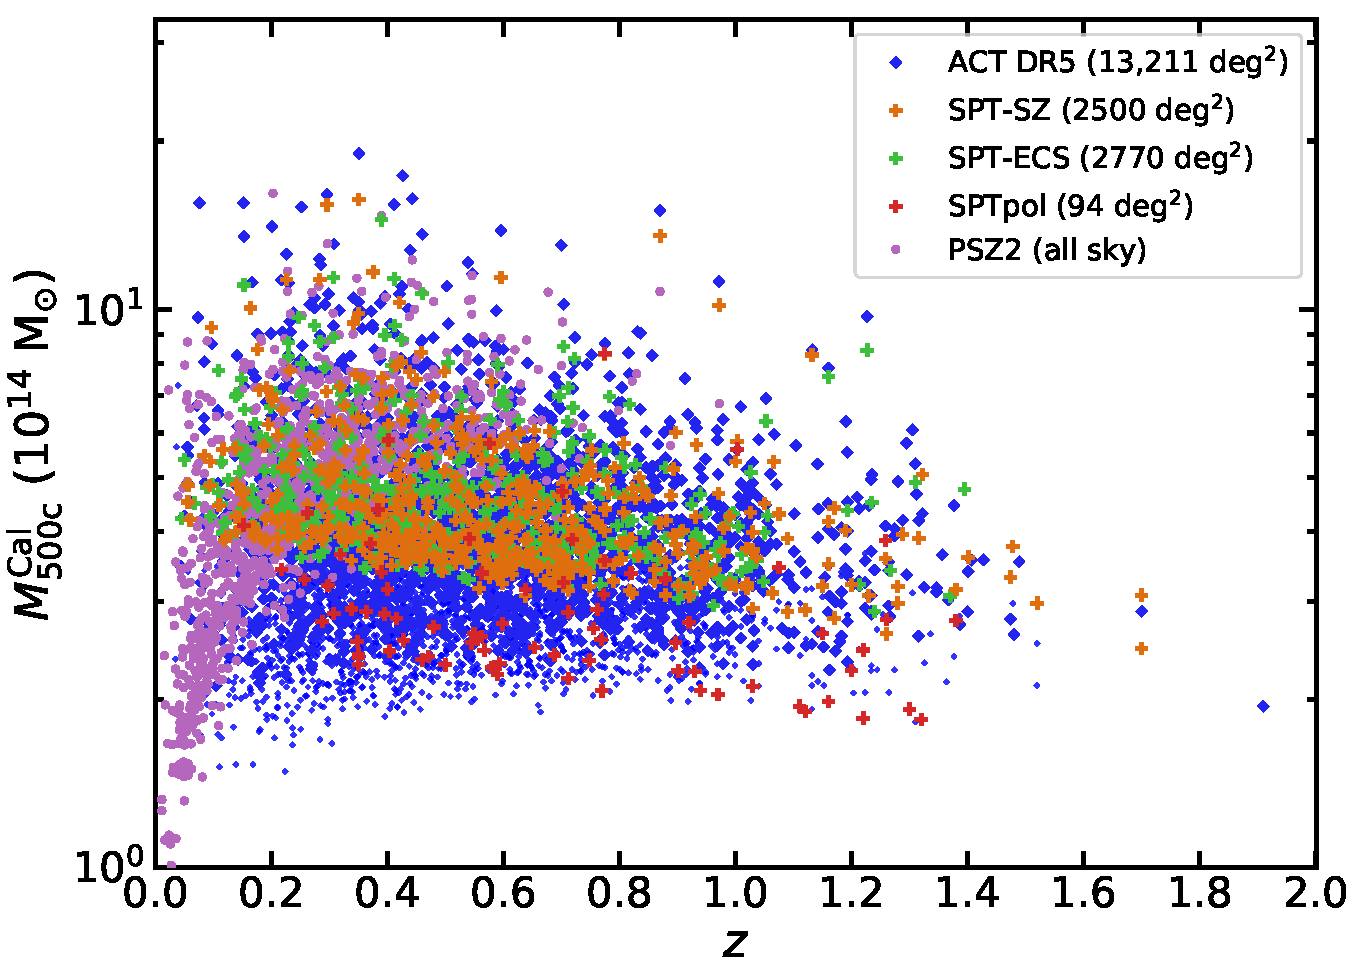
\includegraphics[width=.6\textwidth]{Figures/Chap_amas/mz_sz.pdf}
    \caption{
        Distribution dans le plan masse-redshift des amas détectés par les relevés ACT (bleu, \cite{hilton_atacama_2021}), SPT (orange \cite{bleem_galaxy_2015}, vert \cite{bleem_sptpol_2020} et rouge \cite{huang_galaxy_2020}) et \textit{Planck} (violet, \cite{planck_collaboration_planck_2016-1}).
        Figure extraite de \cite{hilton_atacama_2021}.
    }
    \label{fig:cluster_catalogs_mz}
\end{figure*}

Ces catalogues ont pu être utilisés pour contraindre les paramètres cosmologiques grâce à la distribution des amas en masse et en redshift.
La figure \ref{fig:cluster_S8} montre les contraintes apportées par chacun de ces relevés sur la combinaison de paramètres $S_8 \equiv \sigma_8 \sqrt{\Omega_m/0.3}$, discutée en section \mypageref{sec:cosmo_hmf}.
Les mesures de ce paramètre par des analyses des anisotropies primaires du CMB et de la distribution des galaxies sont également présentées à titre de comparaison.
Si les résultats apparaissent globalement en accord, à l'exception du comptage d'amas dans le Dark Energy Survey \cite{des_collaboration_dark_2020}, les sondes basées sur l'Univers récent semblent favoriser des valeurs plus basses de $S_8$ que le CMB.

Ce constat, en parallèle avec la tension entre le CMB et les autres sondes dans les mesures du taux d'expansion de l'Univers (\eg\ \cite{riess_large_2019,wong_h0licow_2020,efstathiou_h0_2021}), souligne la nécessité de l'étude des effets systématiques affectant l'inférence des paramètres cosmologiques.
En effet, si une différence dans la mesure des paramètres cosmologiques par des sondes différentes peut être révélatrice de nouvelle physique (\eg\ inhomogénéité de l'Univers \cite{bohringer_observational_2020}, modèles d'énergie sombre interactive \cite{di_valentino_interacting_2020}, neutrinos massifs \cite{bolliet_including_2020} ou gravité modifiée \cite{cataneo_tests_2018}), elle peut également traduire une incompréhension des diverses incertitudes entrant en jeu lors des analyses.
Il est donc crucial d'étudier les possibles effets systématiques affectant les analyses cosmologiques afin de pouvoir évaluer la significativité des tensions et la probabilité qu'elles soient dues à de nouveaux phénomènes.

\begin{figure*}[t]
    \centering
    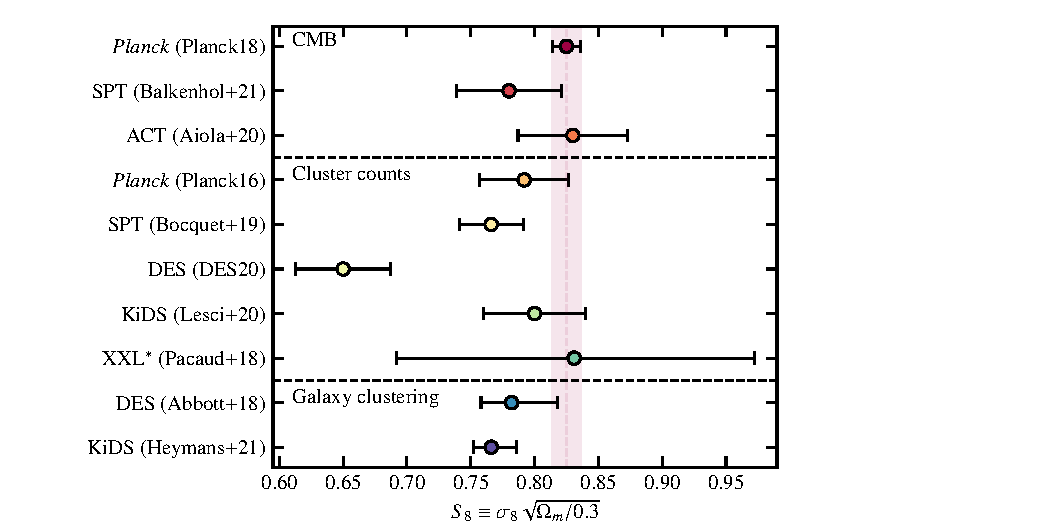
\includegraphics[width=.9\linewidth]{Figures/Chap_amas/S8.pdf}
    \caption{
        Contrainte sur la combinaison de paramètres cosmologiques $S_8$ obtenues par différentes mesures du CMB (haut), de comptage d'amas (milieu), et de distribution de galaxies (bas).
        De haut en bas, les résultats sont issus de \cite{planck_collaboration_planck_2020}\cite{balkenhol_constraints_2021}\cite{aiola_atacama_2020}\cite{planck_collaboration_planck_2016-2}\cite{bocquet_cluster_2019}\cite{des_collaboration_dark_2020}\cite{lesci_amico_2020}\cite{pacaud_xxl_2018}\cite{abbott_dark_2018}\cite{heymans_kids-1000_2021}. \\
        $^*$: incertitudes estimées graphiquement.
    }
    \label{fig:cluster_S8}
\end{figure*}

% ------------------------------------------------------------------------------------- %
\subsection{Relevés futurs}

Les décennies à venir promettent l'essor de la cosmologie avec des amas de galaxies, avec la réalisation d'un grand nombre de relevés du ciel, dans les longueurs d'onde de détection des amas, et avec une qualité de données sans précédent.

En optique, les relevés du Vera Rubin observatory et des satellites \textit{Euclid} et \textit{Roman} permettront la détection de centaines de milliers d'amas, avec des résolutions et des profondeurs permettant l'auto-étalonnage en masse à l'aide de lentillage faible jusqu'à haut redshift ($z \sim 2$, \eg\ \cite{lsst_science_collaboration_lsst_2009, sartoris_next_2016}).
En X, le relevé eROSITA anticipe la détection d'environ dix mille amas jusqu'à $z \sim 2$ \cite{merloni_erosita_2012}.
Enfin, en millimétrique, le Simons Observatory prévoit également la détection par effet SZ de $\sim 10^5$ amas, jusqu'à des redshifts $z \sim 3$, pouvant être exploité par auto-étalonnage de masse grâce au lentillage du CMB \cite{ade_simons_2019, louis_calibrating_2017}, et sera supplanté par CMB-S4 \cite{abazajian_cmb-s4_2016}.

Ainsi, les analyses cosmologiques basées sur les amas de galaxies bénéficieront très prochainement d'une grande diminution des incertitudes statistiques.
Dans ce cadre, les effets systématiques déjà importants deviendront dominants, et leur étude cruciale pour l'obtention de résultats compétitifs avec les autres sondes cosmologiques.
En effet, toute méconnaissance des outils nécessaires aux analyses cosmologiques, comme les relations d'échelle masse-observable, la forme de la fonction de masse, ou le profil de pression moyen des amas\footnote{discuté au chapitre suivant}, aura un impact sur les paramètres cosmologiques qui pourra ne plus être négligeable devant les effets statistiques (\eg\ \cite{ruppin_impact_2019, salvati_impact_2020, artis_impact_2021}).
Il sera alors important de maîtriser ces systématiques pour pouvoir tirer pleinement parti des jeux de données à venir.

% ------------------------------------------------------------------------------------- %
\subsection{Suivis dédiés d'échantillons d'amas}\label{sec:follow_ups}

Toute observation astronomique doit faire face à un compromis entre qualité des observations d'objets individuels et nombre d'objets détectés.
Dans le cadre des amas de galaxies, ce compromis permet de distinguer deux grandes catégories d'observations.
D'une part, les relevés d'amas sont basés sur l'observation homogène d'une portion du ciel, puis sur la détection des objets présents dans les observations.
Ils permettent l'établissement de grands catalogues nécessaires aux analyses cosmologiques comme le comptage d'amas, mais les données qui en sont issues ne permettent en général pas l'étude détaillée des propriétés physiques des amas.
Par exemple, dans le cas de l'effet SZ, le relevé \textit{Planck} \cite{planck_collaboration_planck_2016-2} a été réalisé avec une basse résolution angulaire de l'ordre de 7 arcmin.
Celle-ci ne permettant pas de résoudre les amas lointains, l'étude des propriétés thermodynamiques des amas individuels avec \textit{Planck} est limitée aux objets proches.
Or, la connaissance de ces propriétés est nécessaire aux analyses cosmologiques; aussi, une évolution de celles-ci avec le redshift, indétectable avec les données \textit{Planck} seules, aurait des conséquences sur les analyses cosmologiques basées sur ce catalogue (\eg\ \cite{ruppin_impact_2019}).

L'incapacité à mener des études détaillées des propriétés des amas à partir des relevés peut être compensée par un autre type d'observations: les suivis dédiés d'amas.
Ceux-ci permettent d'utiliser un instrument dédié à l'observation d'un plus petit nombre d'amas, mais fournissent des informations plus détaillées sur leurs propriétés.
Dans l'exemple de l'effet SZ, des instruments à haute résolution angulaire, comme les caméras NIKA2 \cite{adam_nika2_2018,perotto_calibration_2020} ou MUSTANG2 \cite{dicker_mustang2_2014}, permettent de cartographier l'effet SZ en direction d'amas lointains et d'étudier leurs propriétés thermodynamiques.
L'exemple du grand programme SZ de NIKA2 \cite{mayet_cluster_2020}, au sein duquel s'inscrit le travail effectué au cours de cette thèse, sera détaillé dans le chapitre suivant, en section \mypageref{sec:lpsz}.
Si l'échantillon suivi est représentatif de la population d'amas dans l'Univers, les propriétés observées des amas, comme la relation masse-observable, peuvent être généralisées à un relevé ne fournissant pas une information aussi détaillée.
De tels échantillons permettent donc l'étalonnage des outils nécessaires à la cosmologie sur un nombre restreint d'amas, avec une grande qualité de données, permettant l'étude des effets systématiques affectant les analyses cosmologiques basées sur les relevés d'amas.
Nous reviendrons sur ce point au chapitre \ref{chap:scaling}, dans lequel nous présenterons l'étalonnage de la relation d'échelle masse-observable pour le grand programme SZ de NIKA2.

% ------------------------------------------------------------------------------------- %
\subsection{Conclusions}

Dans ce chapitre, nous avons discuté des propriétés des amas de galaxies et détaillé l'utilisation de leur distribution dans l'Univers comme sonde cosmologique.
Au cours des dernières années, les différences entre les mesures des paramètres cosmologiques effectuées au travers de plusieurs sondes ont mis en évidence la nécessité de la maîtrise des effets systématiques propres aux analyses de chaque sonde.
Dans ce contexte, les amas de galaxies s'imposent comme une opportunité hors pair de maximiser le retour scientifique de chaque relevé du ciel.
En effet, de par la nature multilongueur d'onde de ces objets, la plupart des relevés du ciel sont en mesure de détecter des amas de galaxies: des observations du CMB, pouvant détecter des amas par effet SZ, aux relevés de galaxies, pouvant identifier les amas aux surdensités dans la distribution de ces dernières.
Ainsi, des relevés originellement prévus pour une sonde cosmologique peuvent utiliser les amas pour des résultats indépendants de leur sonde primaire, augmentant le pouvoir contraignant de leurs données sur les paramètres cosmologiques.

Nous avons vu que les relevés du futur permettraient une réduction drastique des incertitudes statistiques associées aux comptage d'amas.
La cosmologie avec des amas de galaxies entre donc dans une ère dans laquelle l'étude des effets systématiques sera cruciale à l'exploitation de relevés d'amas.
À l'heure actuelle, les effets systématiques dominants en cosmologie avec des amas proviennent pour la plupart de la méconnaissance des propriétés des amas et de leur évolution avec le redshift.
Dans ce contexte, la mise en place de suivis d'échantillons d'amas a le potentiel de fournir des études détaillées des effets systématiques liés à la détection et l'exploitation cosmologique des amas.

Les amas de galaxies promettent donc de jouer un rôle majeur dans la cosmologie des années à venir, et l'étude détaillée de leurs propriétés permettra d'augmenter leur potentiel en tant que sonde cosmologique.
